\section{DataMCComparison}
\label{sec:DataMCComparison}

The shapes of distributions of the discriminating variables used to separate
out the combinatorial background are compared in data and MC samples.
This analysis is detailed in~\cite{bsmumuv2} [App. A and C].
   
\subsection{Continuum events}
\label{sec:compcont}
  
To check the shapes of the discriminating variables for the
combinatorial background we compare the signal MC sample with
the data sidebands. The signal sample is re-weighted on PV and separately on the \pt\ $^B$, $\eta$ $^B$ and B Isolation
variables simultaneously with a gradient boosted re-weighting technique~\cite{Rogozhnikov:2016bdp}.
Figure~\ref{fig:xcheckcont} shows the corrected \pt\ , $\eta$ ,  and B Isolation variables as a cross-check.
  
Figure~\ref{fig:maincompcont} shows the distributions of few
discriminating variables. The rest can be checked in
\yel[t.b.d.]{Appendix}~\ref{app:contBDT}.
  
\begin{figure}[!htb]
\begin{center}
\hspace*{-0.6cm}
% 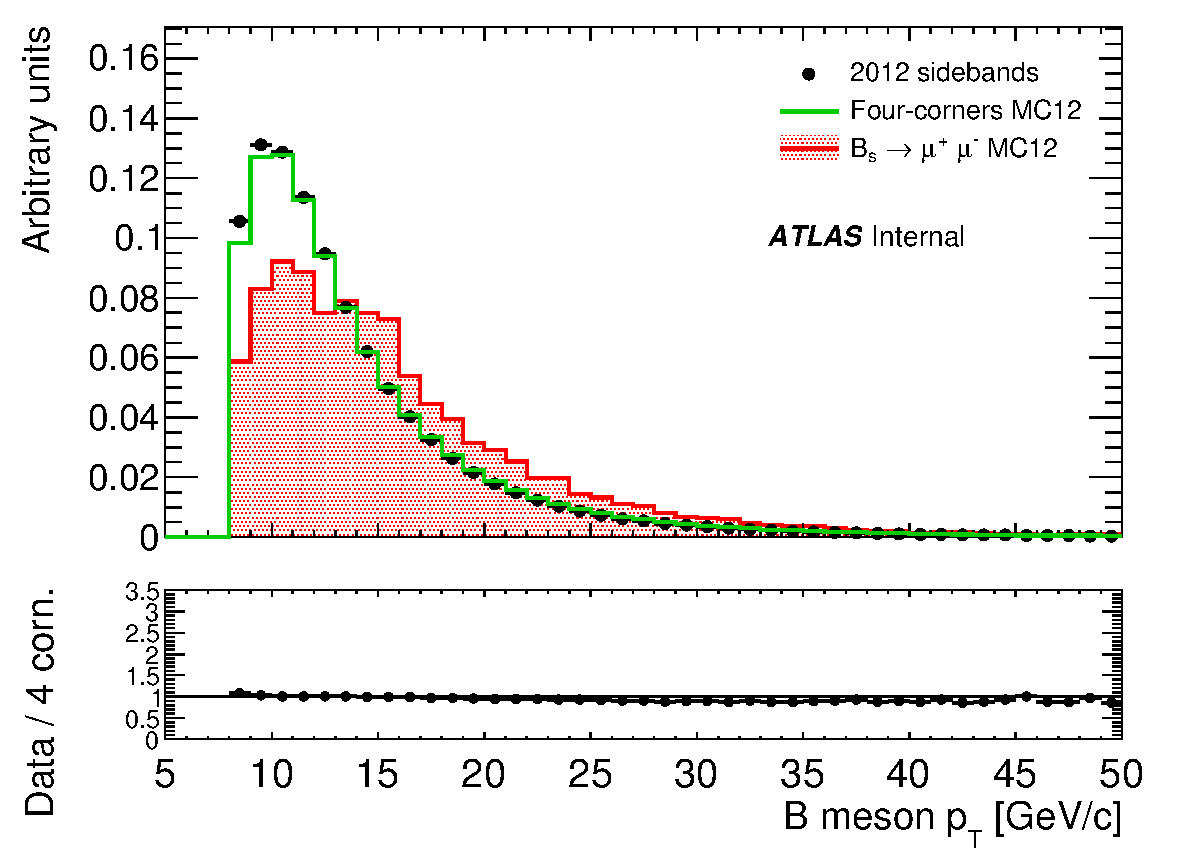
\includegraphics[width=0.52\textwidth]{figures/InternalNote_DataMCComparison/compRun1/cont/pT_data4corn_reweighted.pdf}
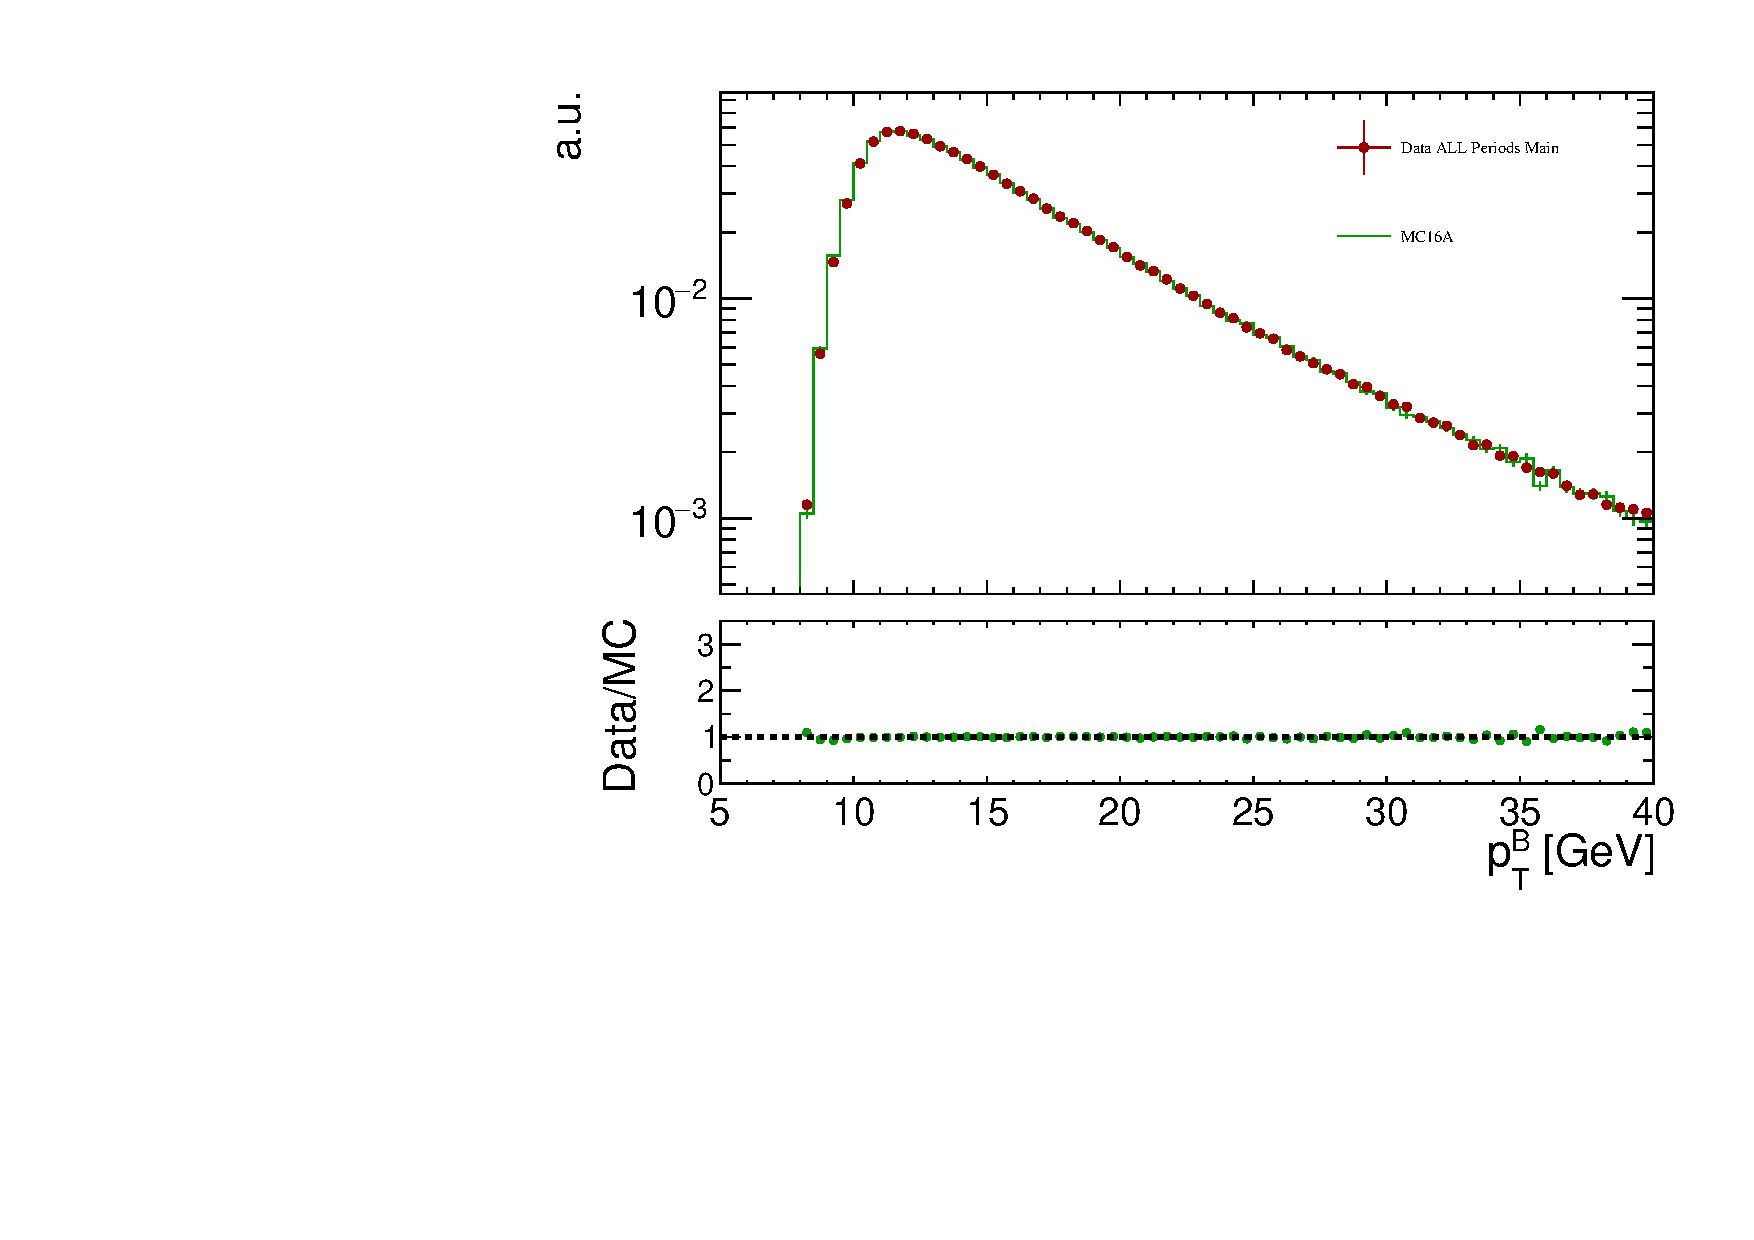
\includegraphics[width=0.52\textwidth]{figures/InternalNote_DataMCComparison/comp/B_pT_dt_mcXs.pdf}
\hspace*{-0.3cm}
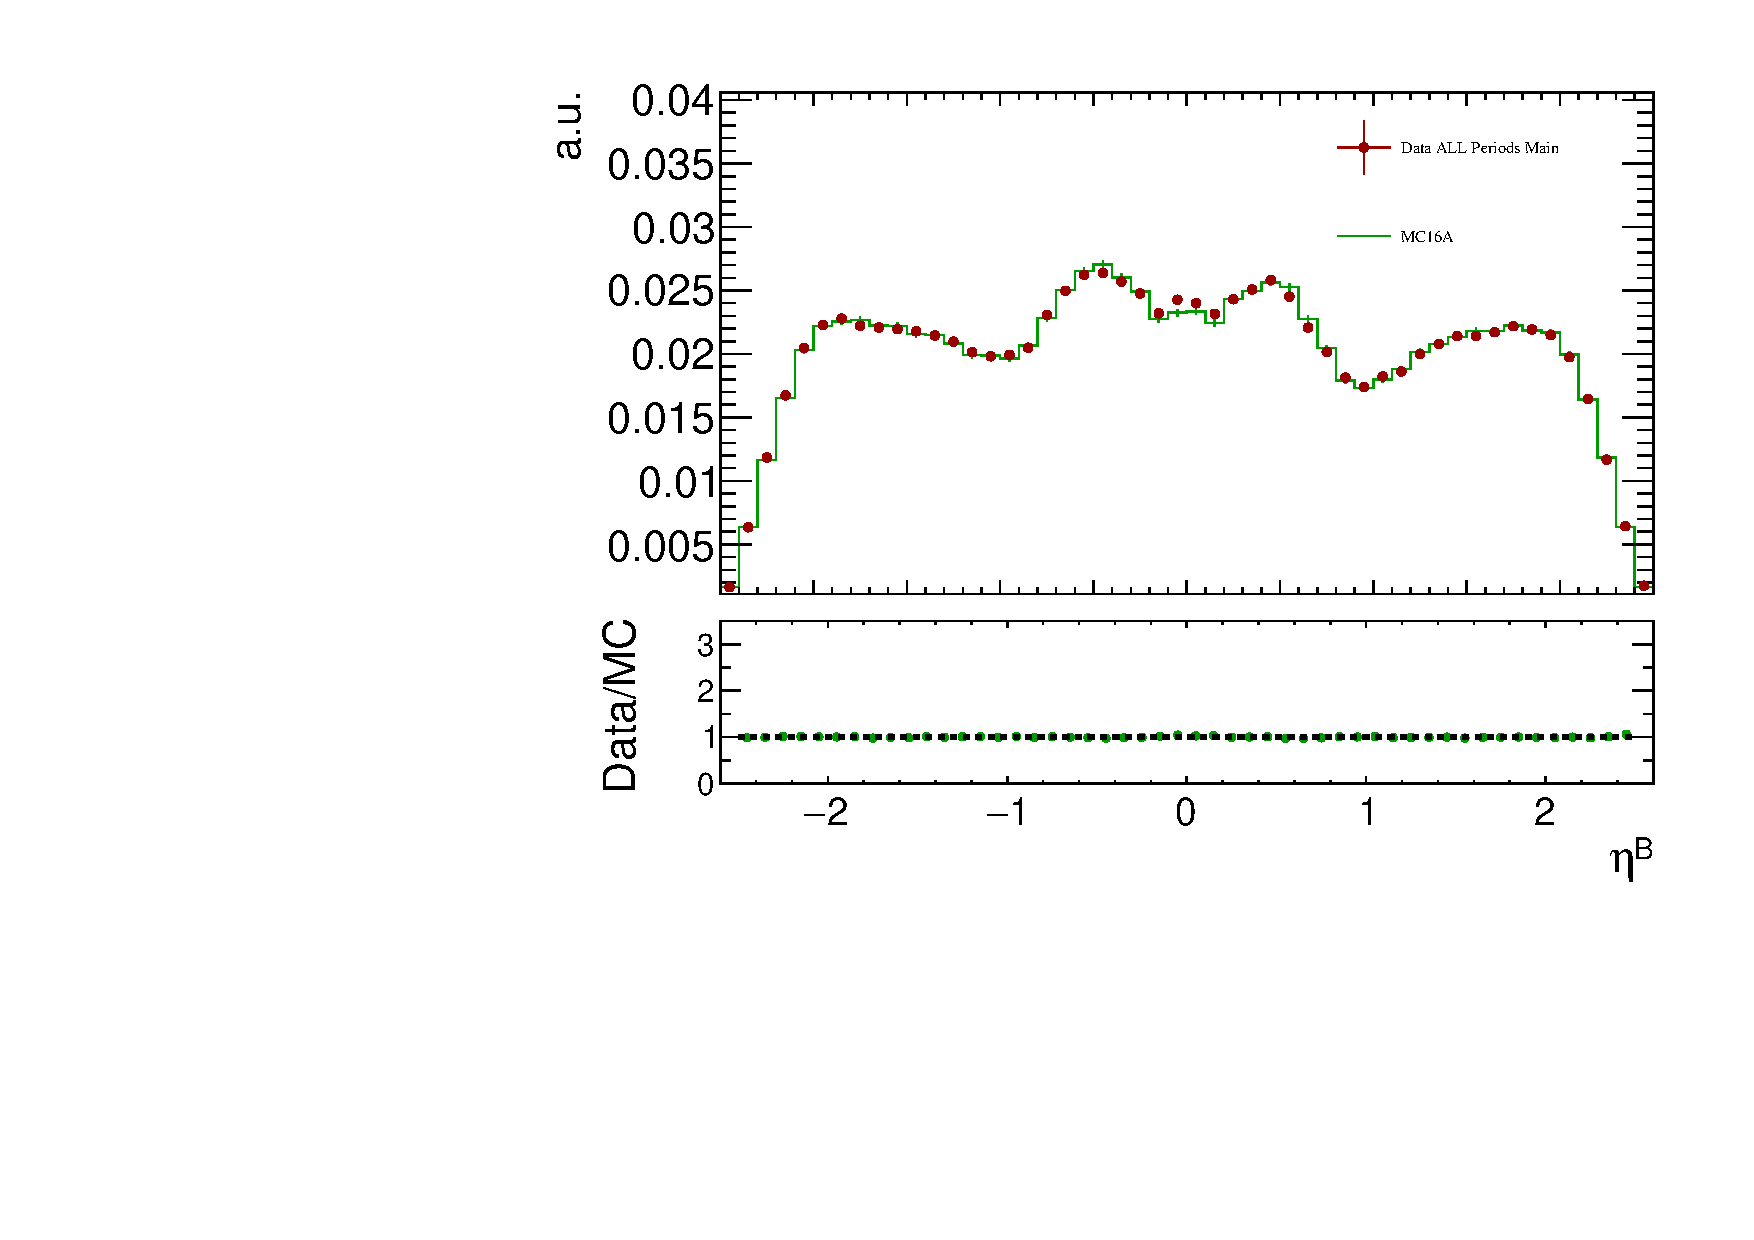
\includegraphics[width=0.47\textwidth]{figures/InternalNote_DataMCComparison/comp/B_eta_dt_mcXs.pdf}
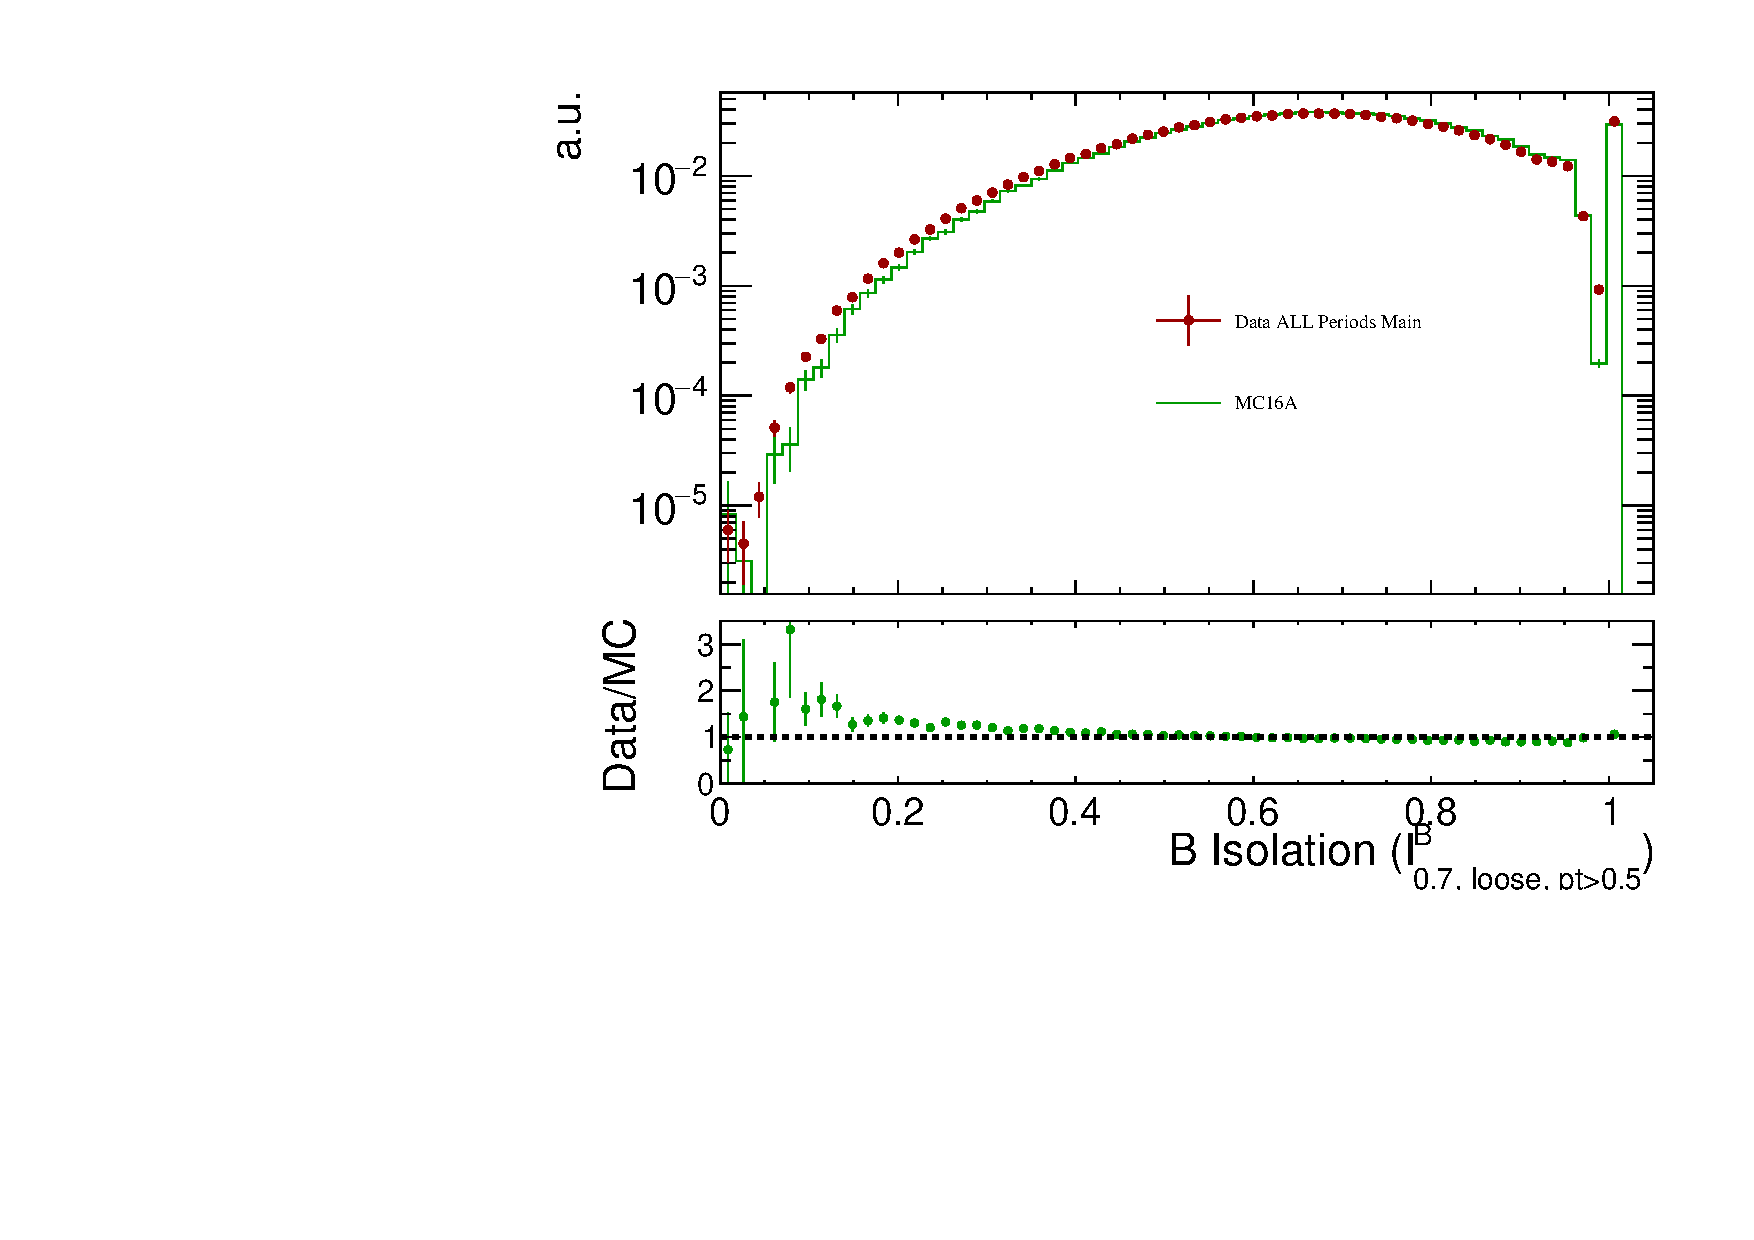
\includegraphics[width=0.52\textwidth]{figures/InternalNote_DataMCComparison/comp/B_iso_7_Chi2_5_LoosePt05_dt_mcXs.pdf}
\caption{Cross-check on the \pt$^B$ and $\eta^B$ distributions of the $J/\psi K$ candidates in data and signal MC.
The red dots correspond to the sideband data during all data taking periods in Run 2 and the green histogram corresponds to the MC $b\bar{b} \to \mu\mu X$ sample. Both histograms are normalised to one.}
\label{fig:xcheckcont}
\end{center}
\end{figure}
%
\begin{figure}[!hbt]
\begin{center}
\hspace*{-0.6cm}
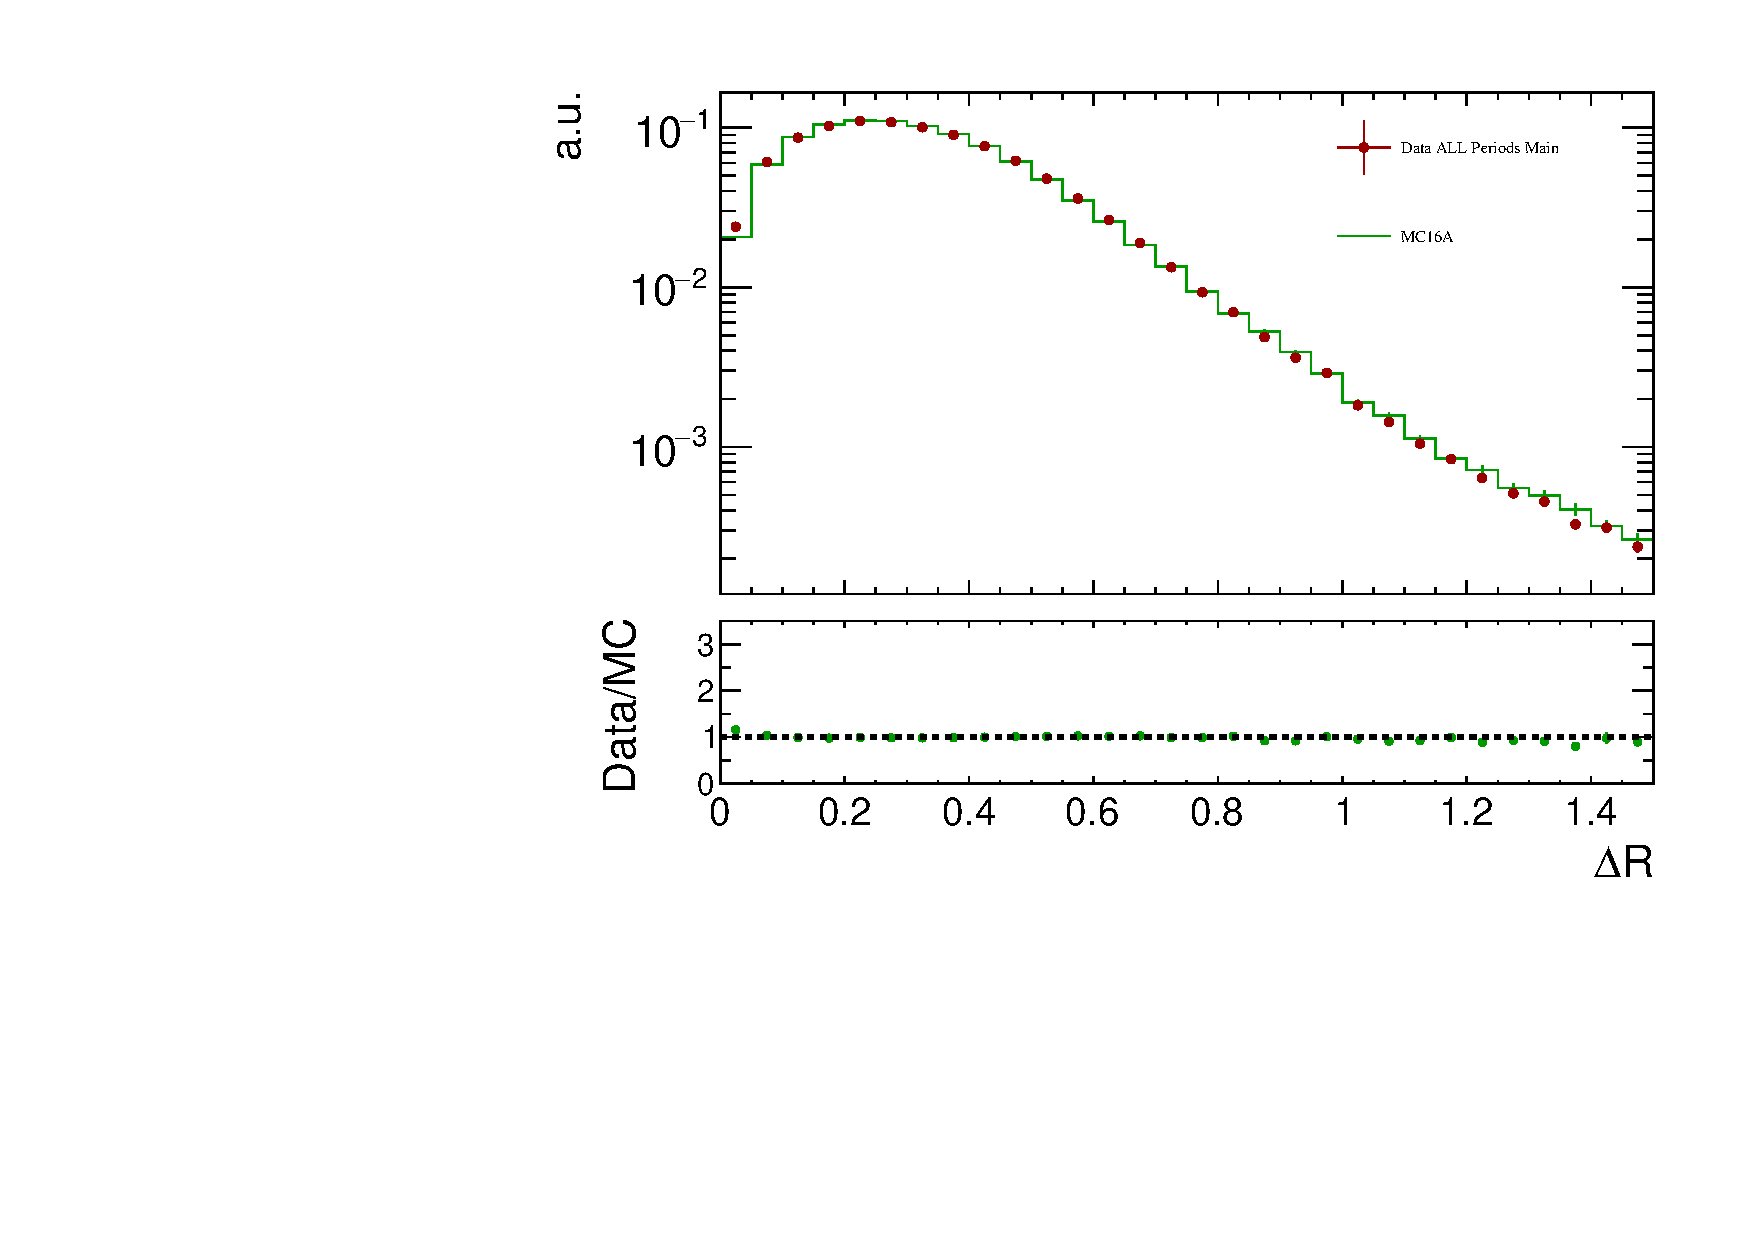
\includegraphics[width=0.52\textwidth]{figures/InternalNote_DataMCComparison/comp/DR_dt_mcXs.pdf}
\hspace*{-0.6cm}
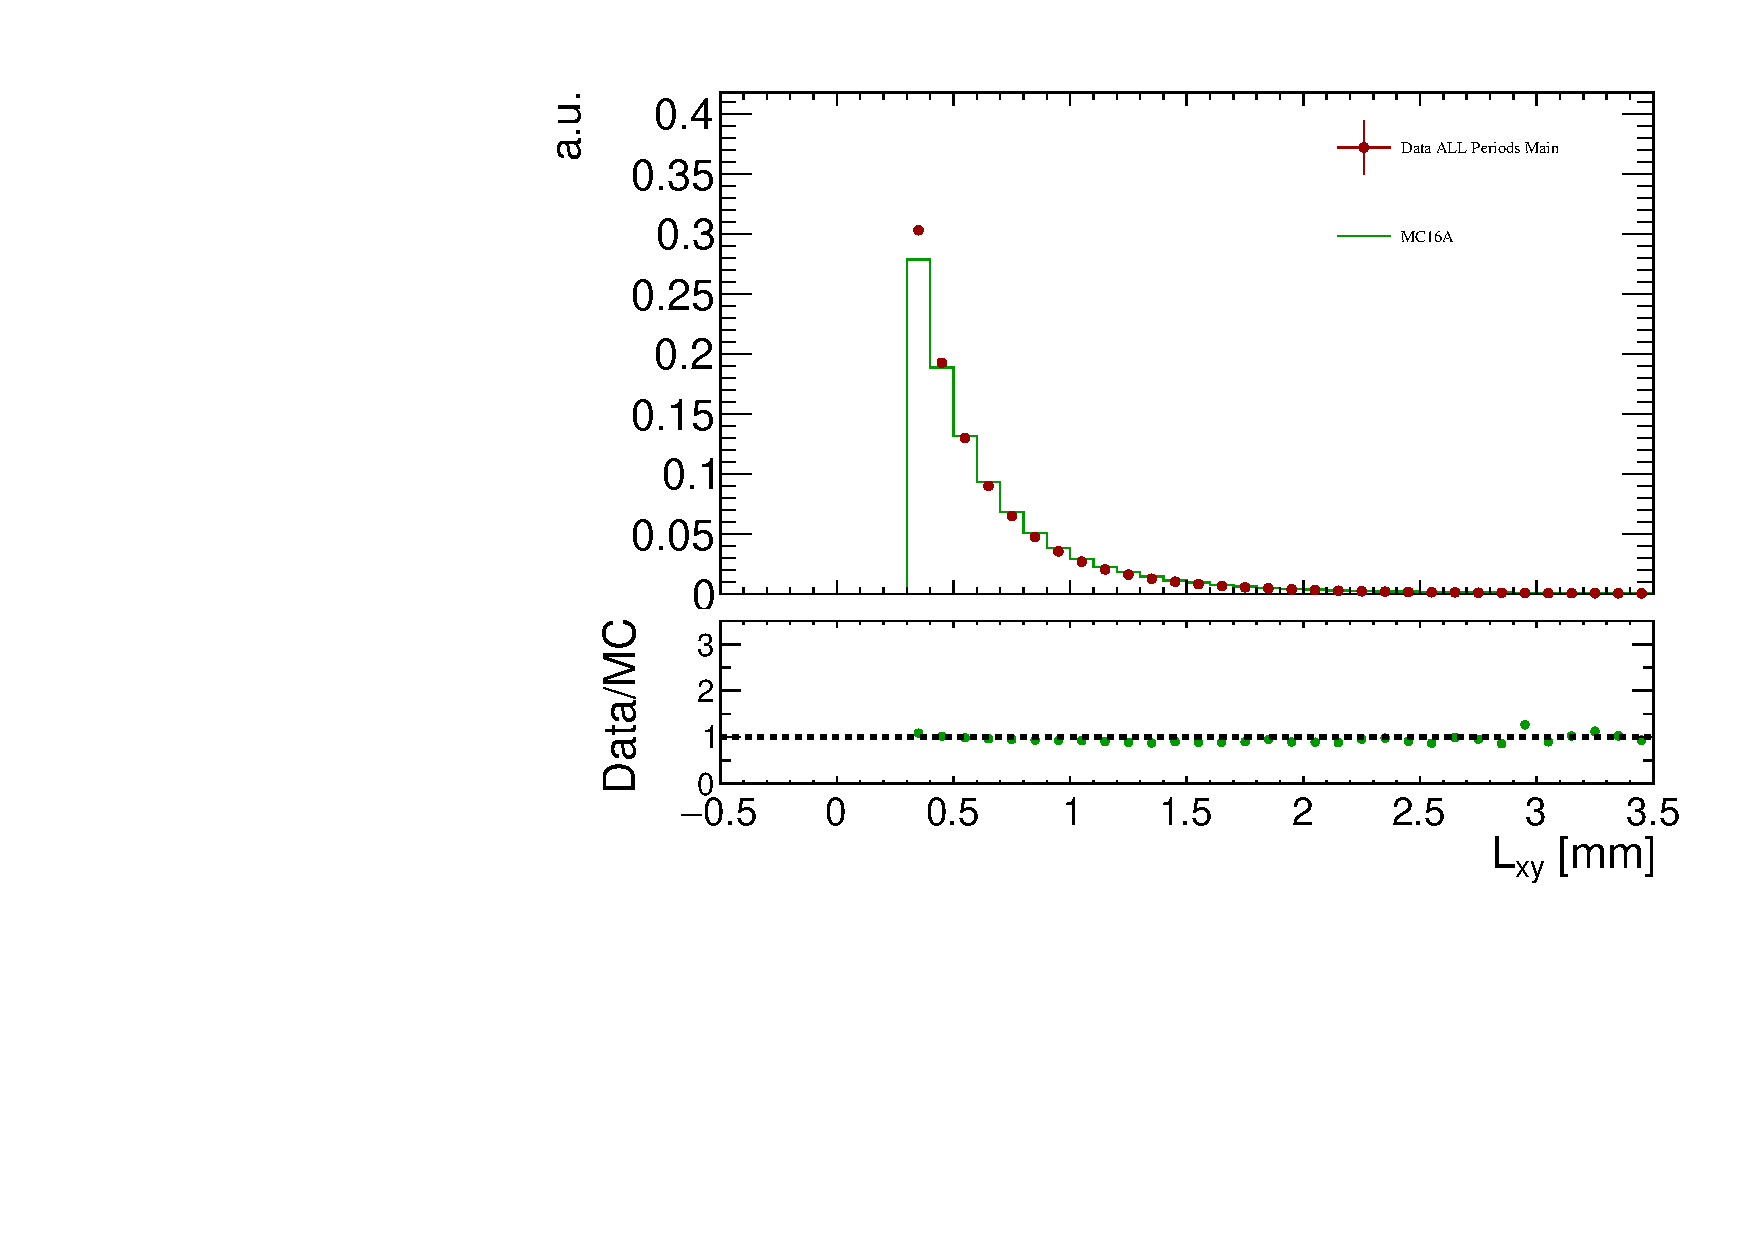
\includegraphics[width=0.52\textwidth]{figures/InternalNote_DataMCComparison/comp/Lxy_dt_mcXs.pdf}\\
\hspace*{-0.6cm}
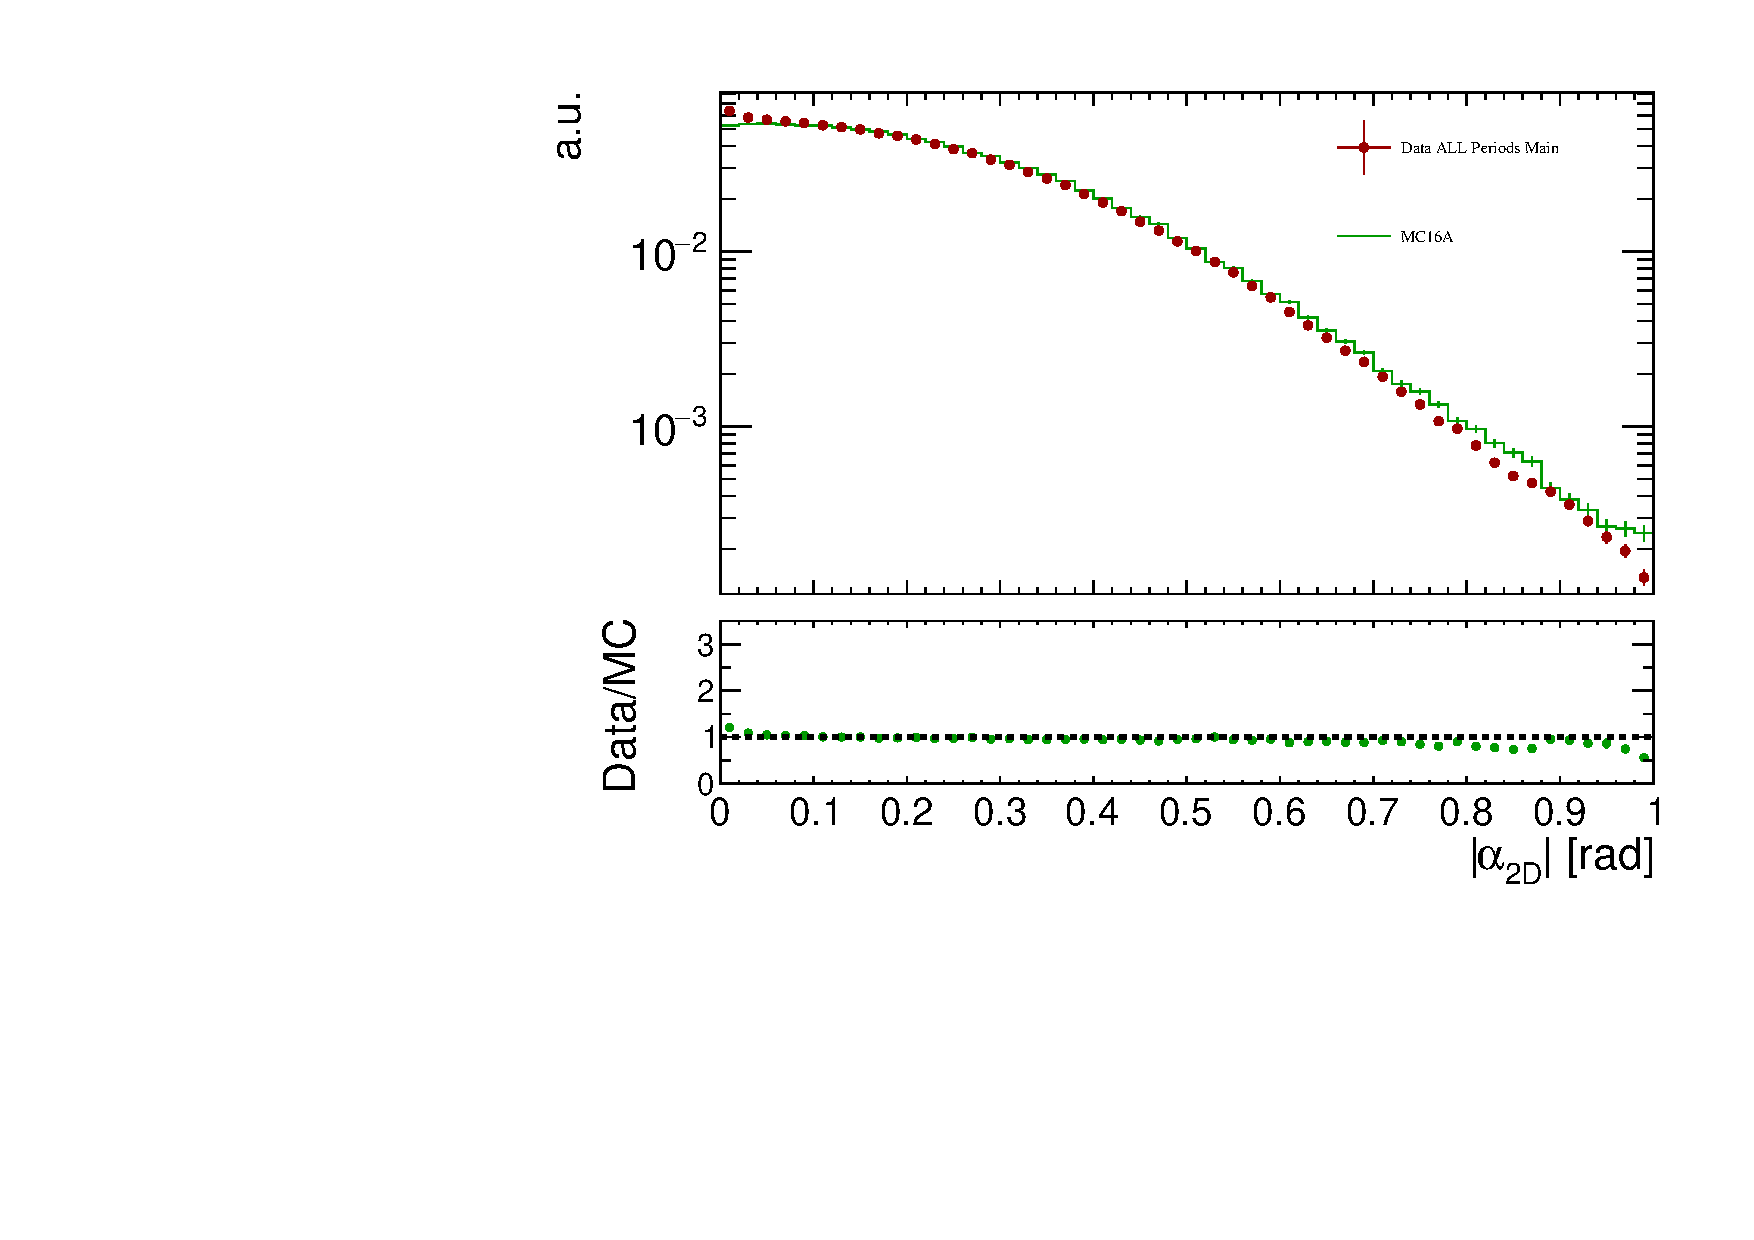
\includegraphics[width=0.52\textwidth]{figures/InternalNote_DataMCComparison/comp/fabs_a_2D__dt_mcXs.pdf}
\hspace*{-0.6cm}
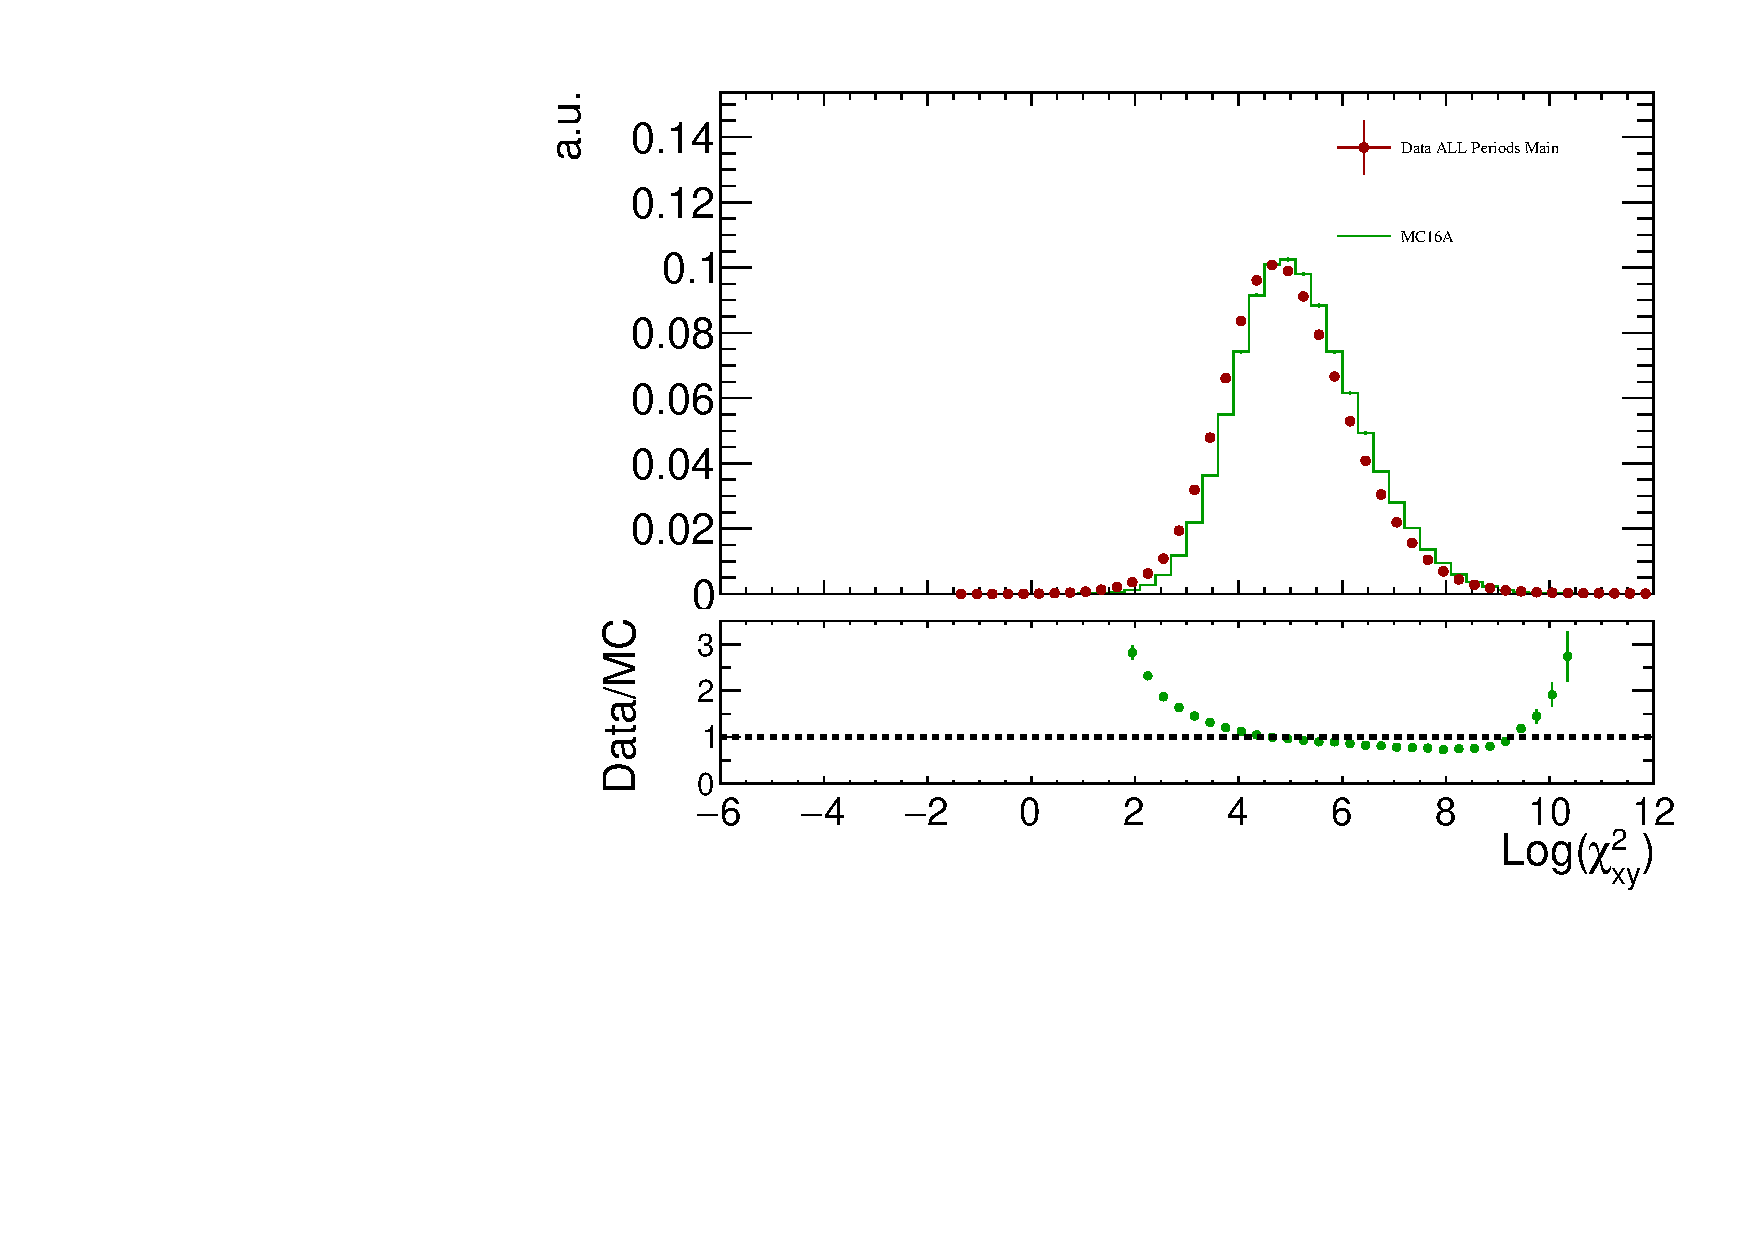
\includegraphics[width=0.52\textwidth]{figures/InternalNote_DataMCComparison/comp/chi2_PVSV_log2D_dt_mcXs.pdf}
\caption{
From left to right, from top to bottom:
Data and signal background MC distributions of the $\Delta R$,
the transverse decay length ($L_{xy}$), $|\alpha_{2D}|$ and
$\chi^{2}_{xy}$ that represents the separation between production
(PV) and decay (SV) vertices.
The green histogram corresponds to the sideband data, while
the red points correspond to the re-weighted signal MC.}
\label{fig:maincompcont}
\end{center}
\end{figure}
  
%\begin{figure}[!hbt]
%\begin{center}
%\hspace*{-0.6cm}
%\includegraphics[width=0.52\textwidth]{eps/contBDT/continuumBDT.pdf}
%%\hspace*{-0.3cm}
%%\includegraphics[width=0.52\textwidth]{eps/contBDT/BvtxLxy_dt_mc_sigFull.pdf}
%\caption{Data and 4-corner background MC distribution of the continuum BDT
%variable. The black dots correspond to the sideband data, while
%the green points correspond to \pt\ and PV re-weighted
%4-corner normalised to the number of data events. The red
%dots show the signal MC distribution as comparison.}
%\label{fig:maincompcontBDT}
%\end{center}
%\end{figure}
  
\subsection{Reference channel as control sample for signal: \BpKpJpsi}
\label{sec:compsig}

The MC sample for the reference channel \BpKpJpsi\ is used to compare
the signal MC shapes with the collision data. The MC sample is
\yel[t.b.d. - currently brute-force approach]{re-weighted with the GLC and the DDW} described in Secs.~\ref{sec:glc}
and~\ref{sec:ddw}. For the data sample, the shape of the background
distribution for each discriminating variable is estimated using the
events falling into the left ($5080\MeV<m_{\Jpsi K^{\pm}}<5180\MeV$)
and the right ($5380\MeV<m_{\Jpsi K^{\pm}}<5480\MeV$) sidebands.

The left sideband contains also a fraction of mis-reconstructed decays
that behave signal-like from the point of view of the discriminating
variables. We re-weight the left sideband considering the combinatorial
contribution only: the net effect is that some of the signal will be
also subtracted as mis-reconstructed $B$ events.~\footnote{From the
binned fit we extract the number of combinatorial background events
in the left and in the right sidebands (let's call them C and D) and
also in the signal region (let's call it A).
Then we normalise the sideband distributions to A/(C+D), effectively
subtracting the right amount of combinatorial background feeding into
the signal region.}
It is proven that the mis-reconstructed events have the same shape as
the signal in the discriminating variables considered, so no distortion
of the signal shapes is created by this subtraction.

\begin{figure}[!ht]
\begin{center}
\hspace*{-0.6cm}
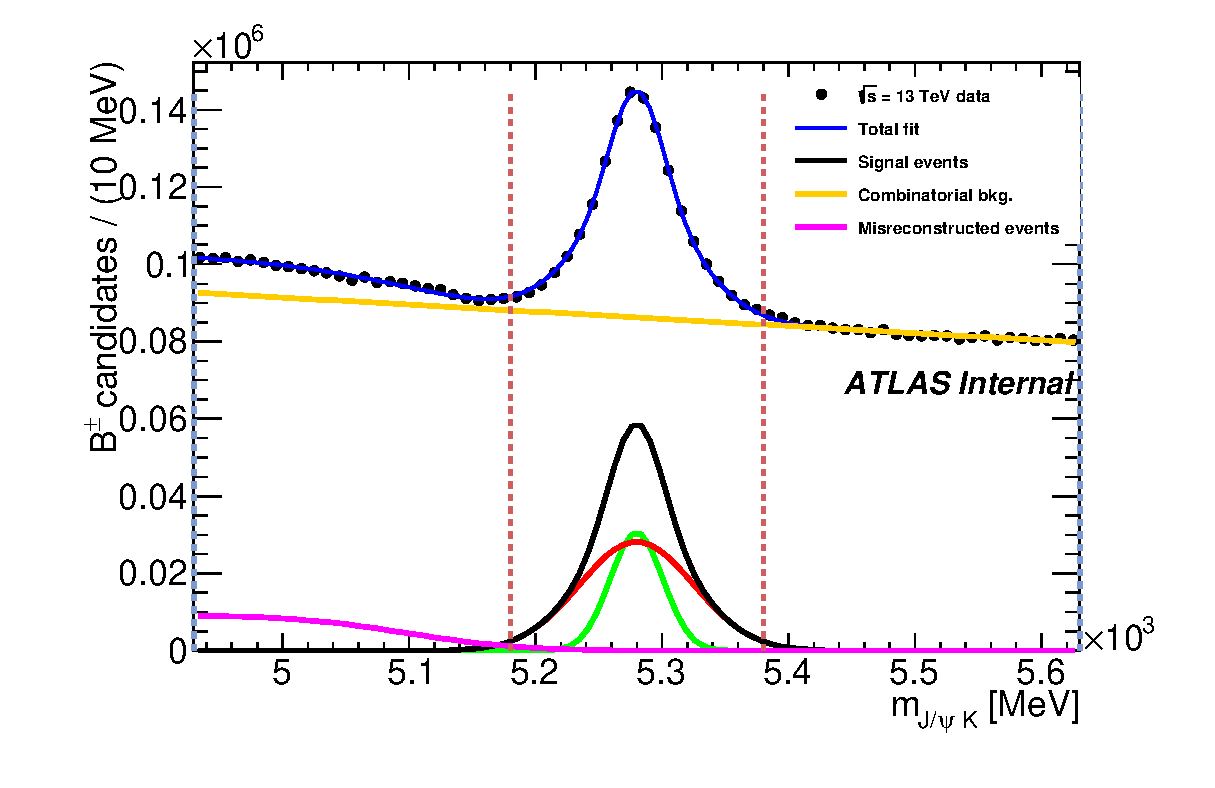
\includegraphics[width=0.47\textwidth]{figures/InternalNote_DataMCComparison/Bp/bplusbinnedfit.eps}
\caption{
Fit to the invariant mass distributions of \BpKpJpsi\ events.}
\label{fig:bplusbinned}
\end{center}
\end{figure}
%
\begin{figure}[!htb]
\begin{center}
\hspace*{-0.6cm}
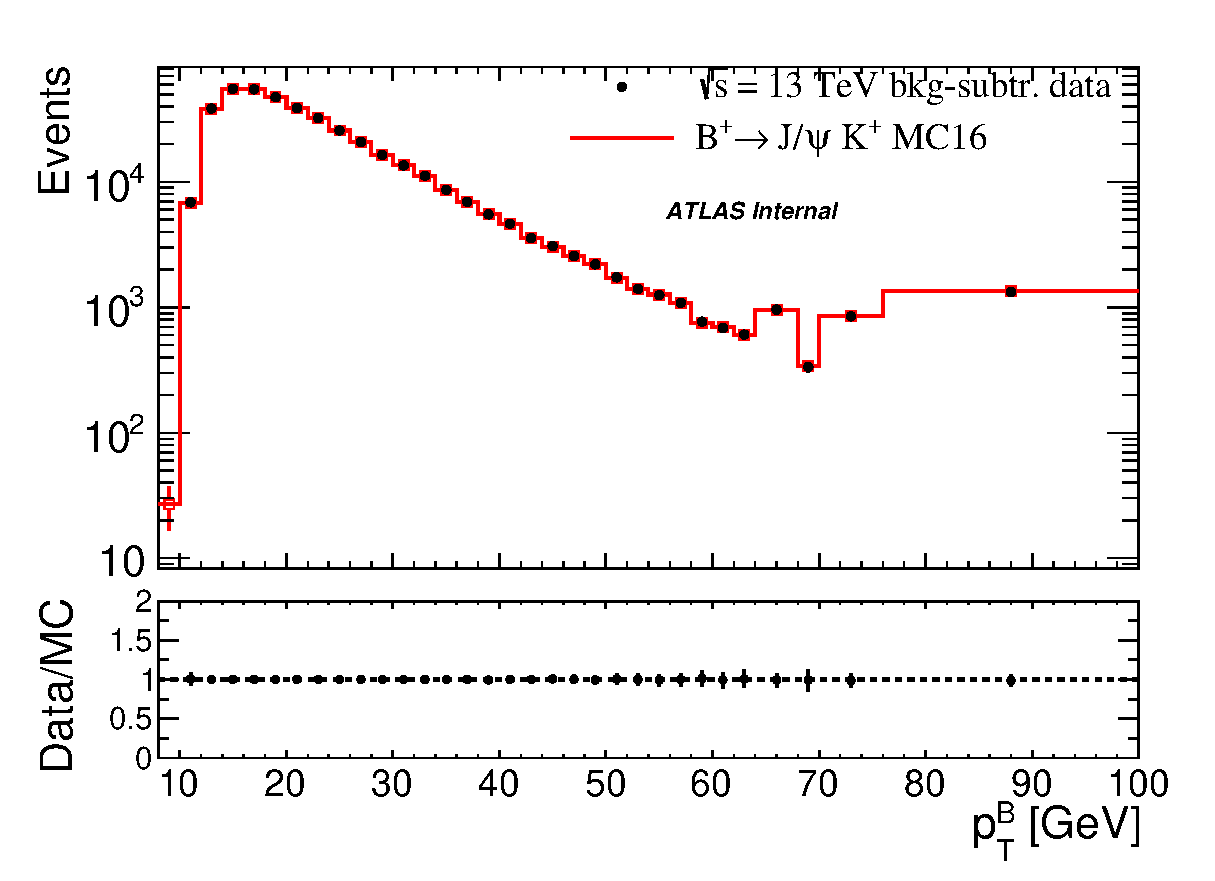
\includegraphics[width=0.52\textwidth]{figures/InternalNote_DataMCComparison/Bp/bplus_pT.eps}
\hspace*{-0.6cm}
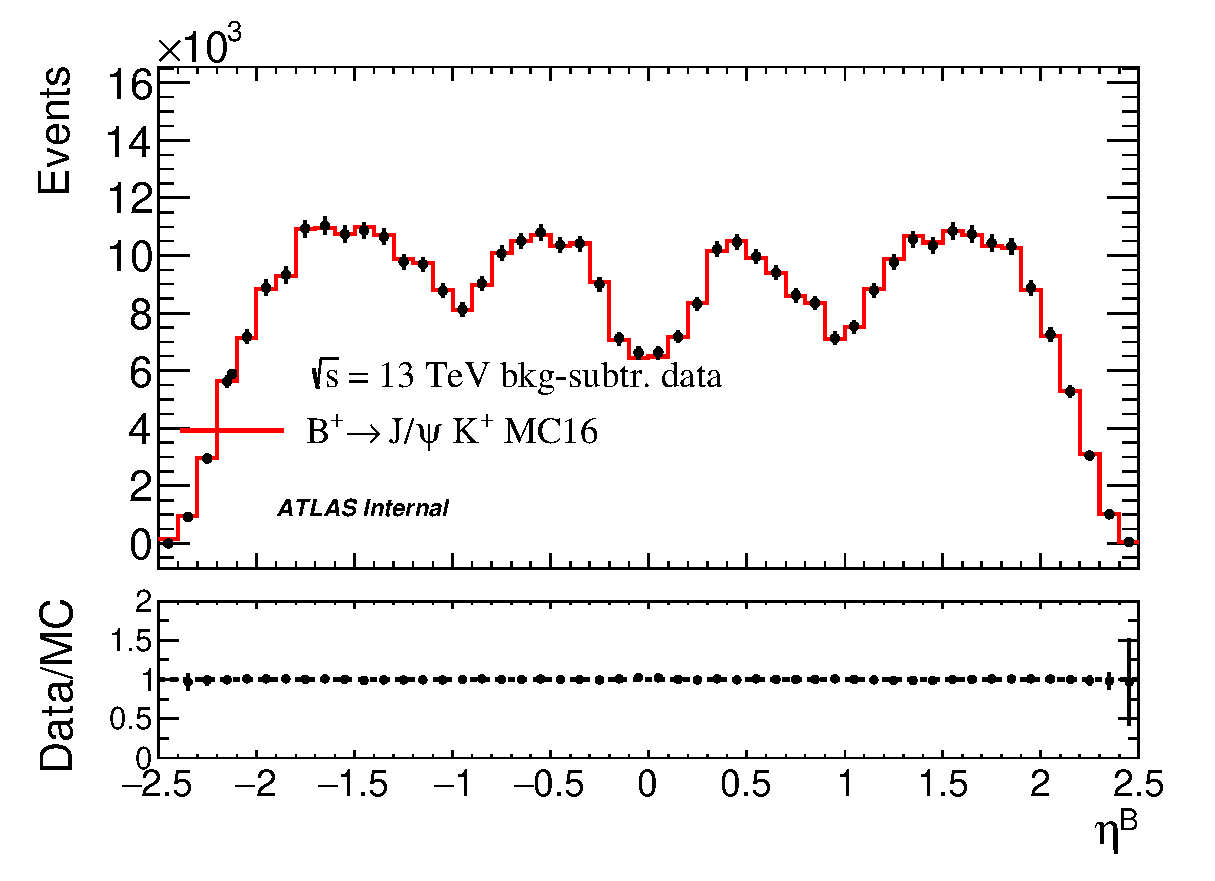
\includegraphics[width=0.52\textwidth]{figures/InternalNote_DataMCComparison/Bp/bplus_eta.eps}
\caption{Cross-check on the \pt$^B$ and $\eta^B$ distributions of
the $J/\psi K$ candidates in data and signal MC.
The black dots correspond to the sideband subtracted data, while 
the red histograms correspond to reweighted MC 
normalised to the number of data events.}
\label{fig:xcheckcompBp}
\end{center}
\end{figure}
%
\begin{figure}[!b]
\begin{center}
\hspace*{-0.4cm}
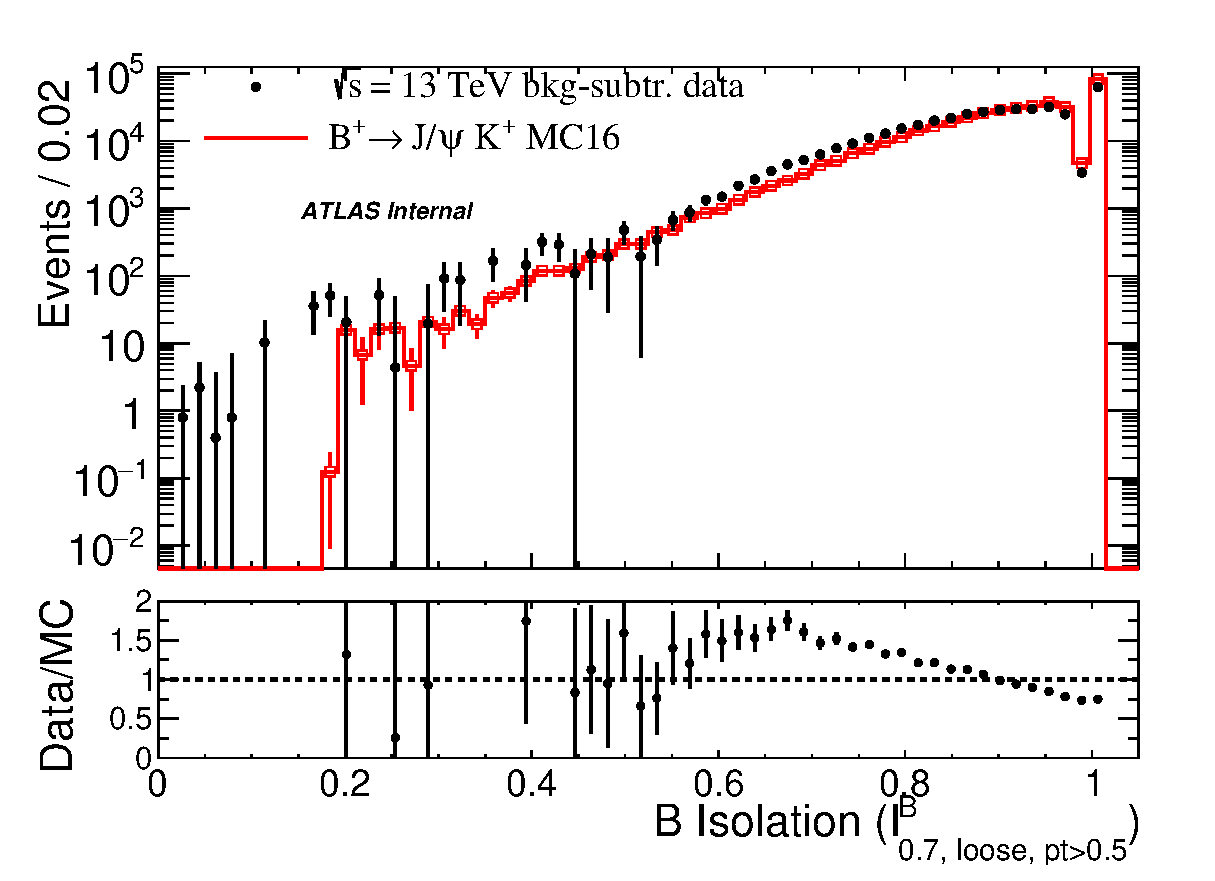
\includegraphics[width=0.47\textwidth]{figures/InternalNote_DataMCComparison/Bp/bplus_iso.eps}
\hspace*{-0.4cm}
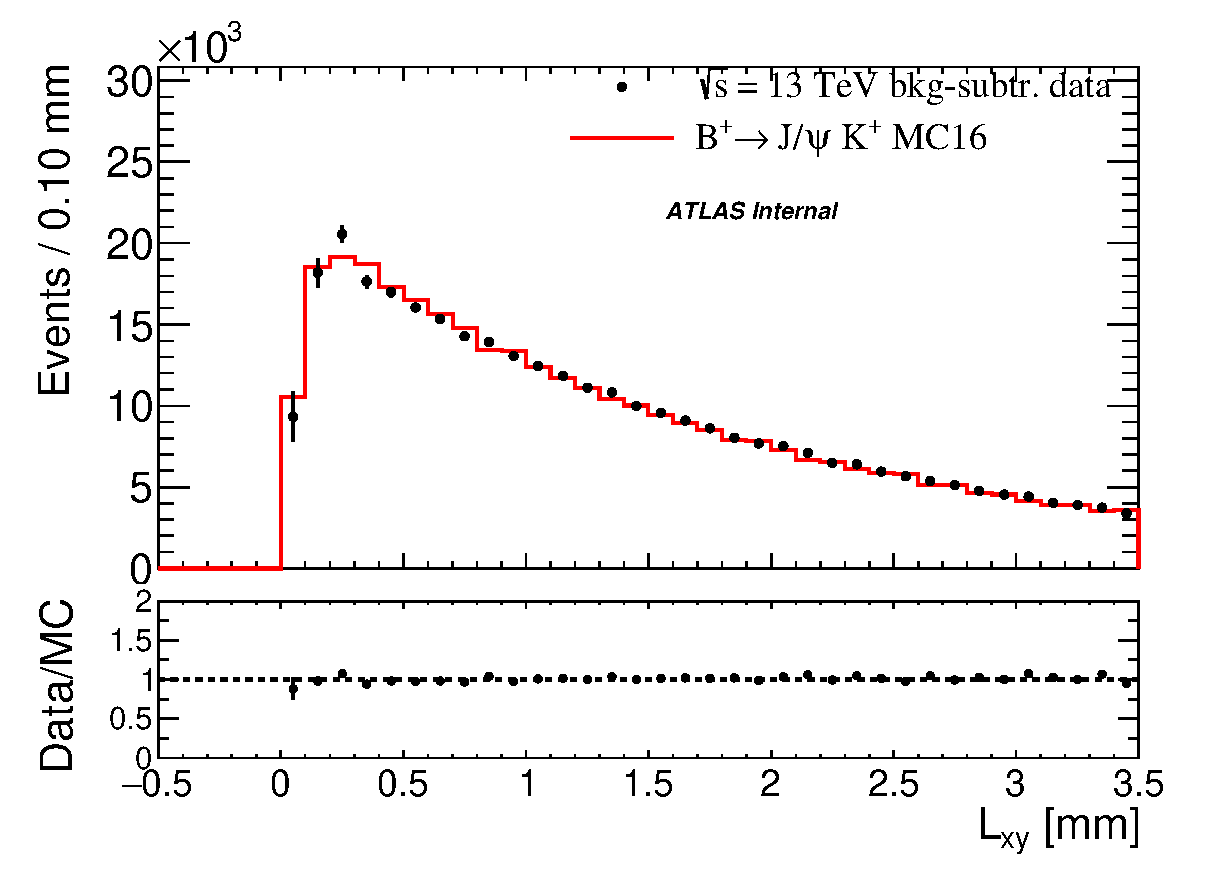
\includegraphics[width=0.47\textwidth]{figures/InternalNote_DataMCComparison/Bp/bplus_Lxy.eps}\\
\hspace*{-0.4cm}
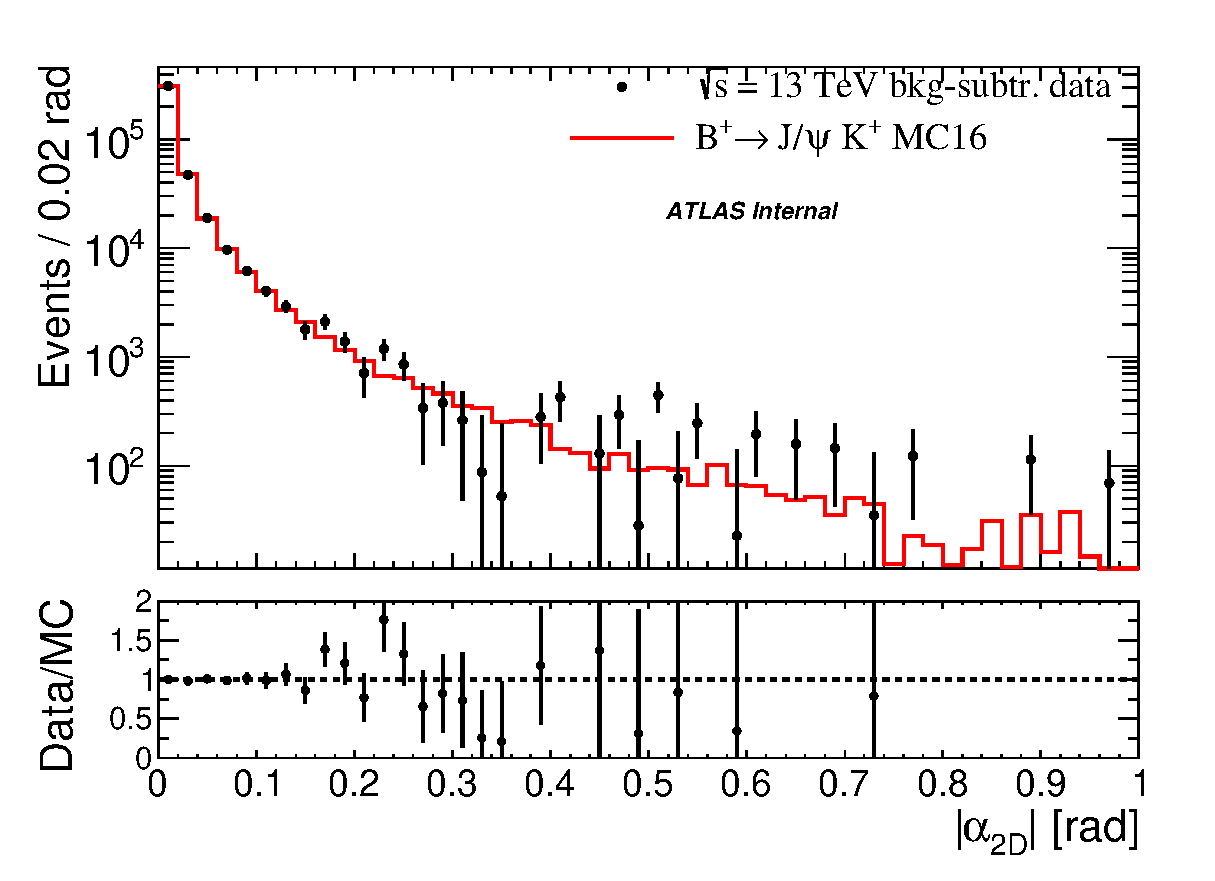
\includegraphics[width=0.47\textwidth]{figures/InternalNote_DataMCComparison/Bp/bplus_a2D.eps}
\hspace*{-0.4cm}
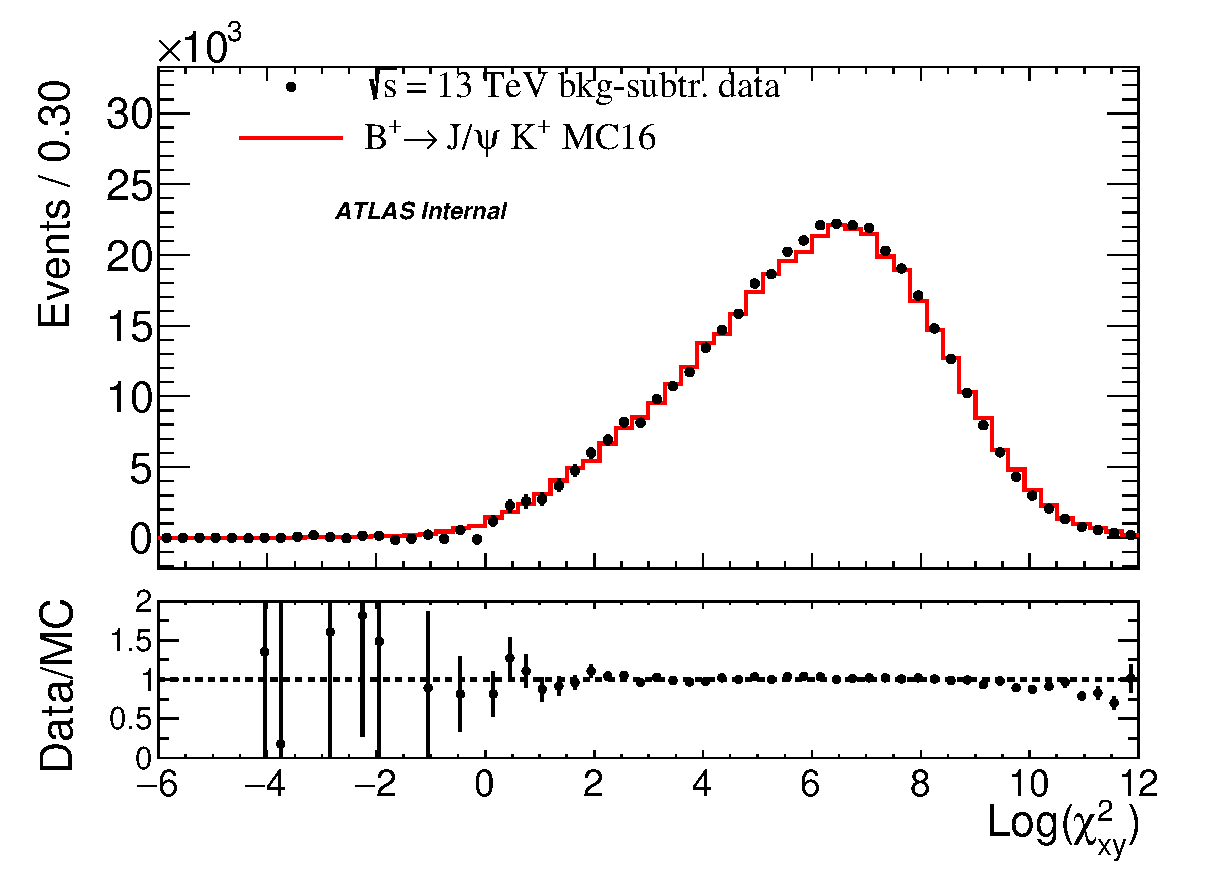
\includegraphics[width=0.47\textwidth]{figures/InternalNote_DataMCComparison/Bp/bplus_chi2PVSV.eps}
\caption{{\it{From left to right, from top to bottom}}: 
Data and signal MC distributions in \BpKpJpsi\ events for the $B$ isolation variable, 
the transverse decay length ($L_{xy}$), $|\alpha_{2D}|$ and 
$\chi^{2}_{xy}$ that represents the separation between production
(PV) and decay (SV) vertices.
The black dots correspond to the sideband subtracted data, while 
the red points correspond to reweighted MC
normalised to the number of data events.}
\label{fig:maincompBp}
\end{center}
\end{figure}
%
\begin{figure}[!b]
\begin{center}
\hspace*{-0.4cm}
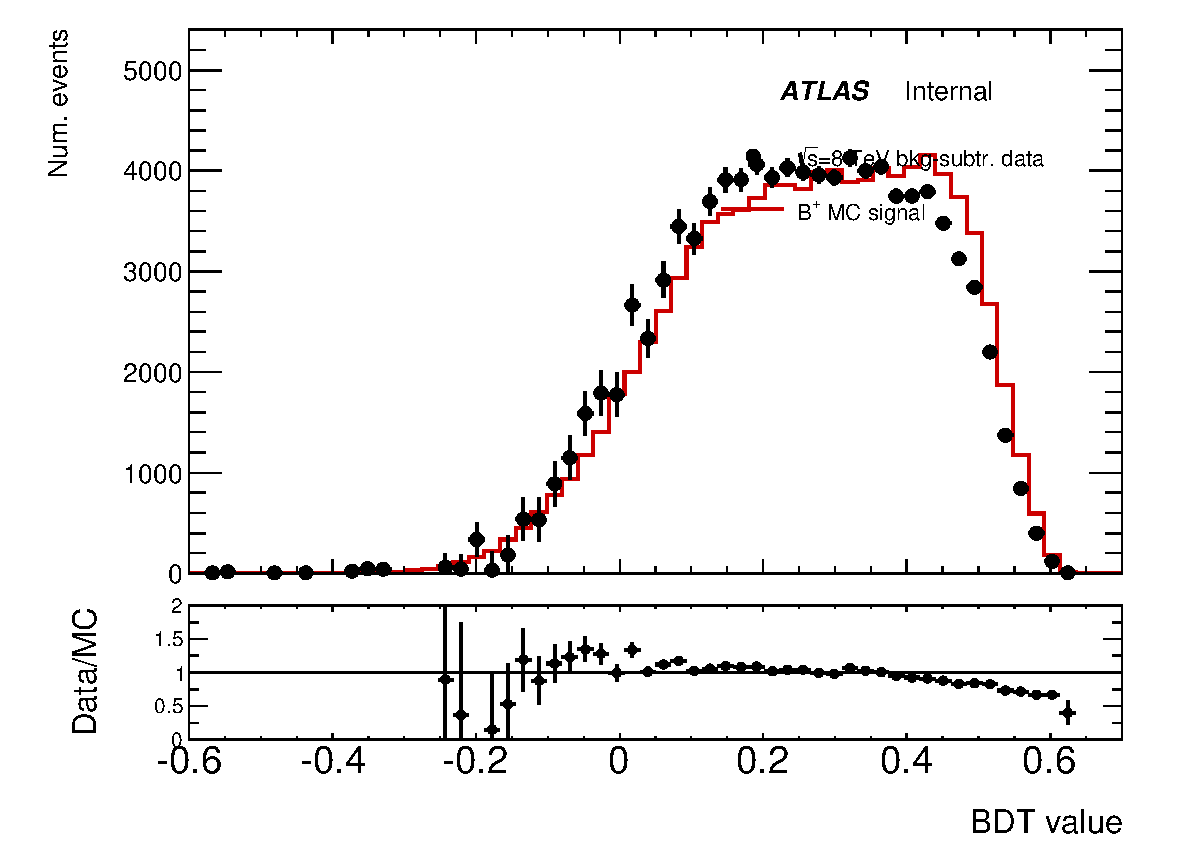
\includegraphics[width=0.47\textwidth]{figures/InternalNote_DataMCComparison/compRun1/Bp/bplus_BDT.pdf}
\hspace*{-0.4cm}
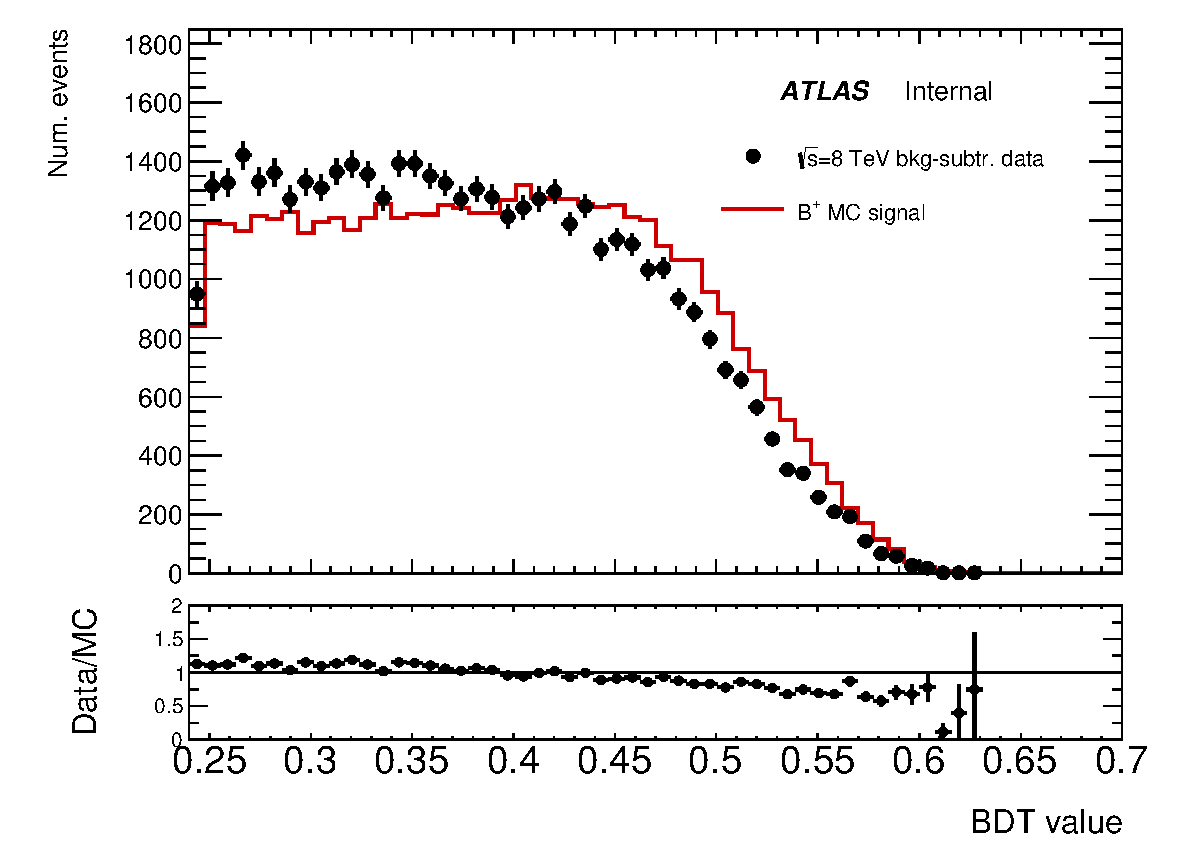
\includegraphics[width=0.47\textwidth]{figures/InternalNote_DataMCComparison/compRun1/Bp/bplus_BDTzoomed.pdf}
\caption{\textbf{Run 1 result, t.b.u.!}Data and signal MC distribution in \BpKpJpsi\ events for the
continuum BDT variable.
The black dots correspond to the sideband subtracted data, while 
the red points correspond to reweighted MC normalised to the number
of data events. The left plot shows the same distribution zoomed
in the region of interest of the analysis.}
\label{fig:maincompBpBDT}
\end{center}
\end{figure}
%
The shape from the rescaled sideband events is subtracted statistically
from the signal region. The number of background events
feeding into the signal region is obtained by a binned
maximum likelihood fit to the mass distribution.
Figure~\ref{fig:bplusbinned} shows these binned fits to
the mass distributions in the three trigger categories.
The fit model consists of a double Gaussian for
the signal, an error function for the
mis-reconstructed events and an exponential for the continuum
background.
The results of these binned fit analysis are perfectly 
compatible with the unbinned fit described in
Section~\ref{sec:bplus} and used for the yield extraction.

The distributions of \pt{} and $\eta{}$ of the $B$ is rechecked in
figures~\ref{fig:xcheckcompBp}, the distributions of few
discriminating variables are shown in figures~\ref{fig:maincompBp},
and \yel[t.b.d.]{the distribution of the continuum BDT variable is shown in
figure}~\ref{fig:maincompBpBDT}.
The distributions of all the other variables are shown in the
\yel[t.b.d.]{appendix}~\ref{app:comp}.

Typically, except for deviations in individual bins, the overall shapes
of distributions agree well between data and MC. The observed differences
in shape are accounted for as systematics with the procedure described in
Section~\ref{sec:eff}. In addition, the discrepancy seen in the
data-MC comparison of the continuum BDT in the \BpKpJpsi\ events is
assessed and exploited in the evaluation of the efficiency in the
\Bsmumu\ signal in Section~\ref{sec:BDTbineff}.

%For this purpose the differences
%for all discriminating variables are calculated per bin and applied to
%the preselected MC events to estimate the impact on the efficiency evaluation
%for systematic studies.% (Appendix~\ref{sec:MVA}). 


\subsection{Alternate reference channel: \BsJpsiPhi}
\label{sec:compjpsiphi}

The same procedure can be applied on data reconstructed as \BsJpsiPhi.
In this case, a few extra selection cuts are necessary to address the extra
kaon in the final state and to select the $\phi$ mass window:
both kaon \pt\ are requested $>1$~GeV and for the $\phi$ mass we require
$|m_{hh}-m_{\phi}|<15$~MeV. The additional cuts defined in
Section~\ref{sec:addcuts} are also applied.
The invariant mass fits in this case are shown in figure~\ref{fig:jpsiphi}
for the three trigger categories.
The fits are performed binned and a Gaussian PDF is used for the signal shape
while a third order Chebychev is used for the combinatorial background PDF.

%\begin{figure}[!htb]
%\begin{center}
%\includegraphics[width=0.37\textwidth]{figures/InternalNote_DataMCComparison/compRun1/Bs/bsjpsiphi_massfit.pdf}
%\caption{Fit to the invariant mass distributions
%of \BsJpsiPhi\ events.}
%\label{fig:jpsiphi}
%\end{center}
%\end{figure}

\begin{figure}[!htb]
\begin{center}
\hspace*{-1cm}
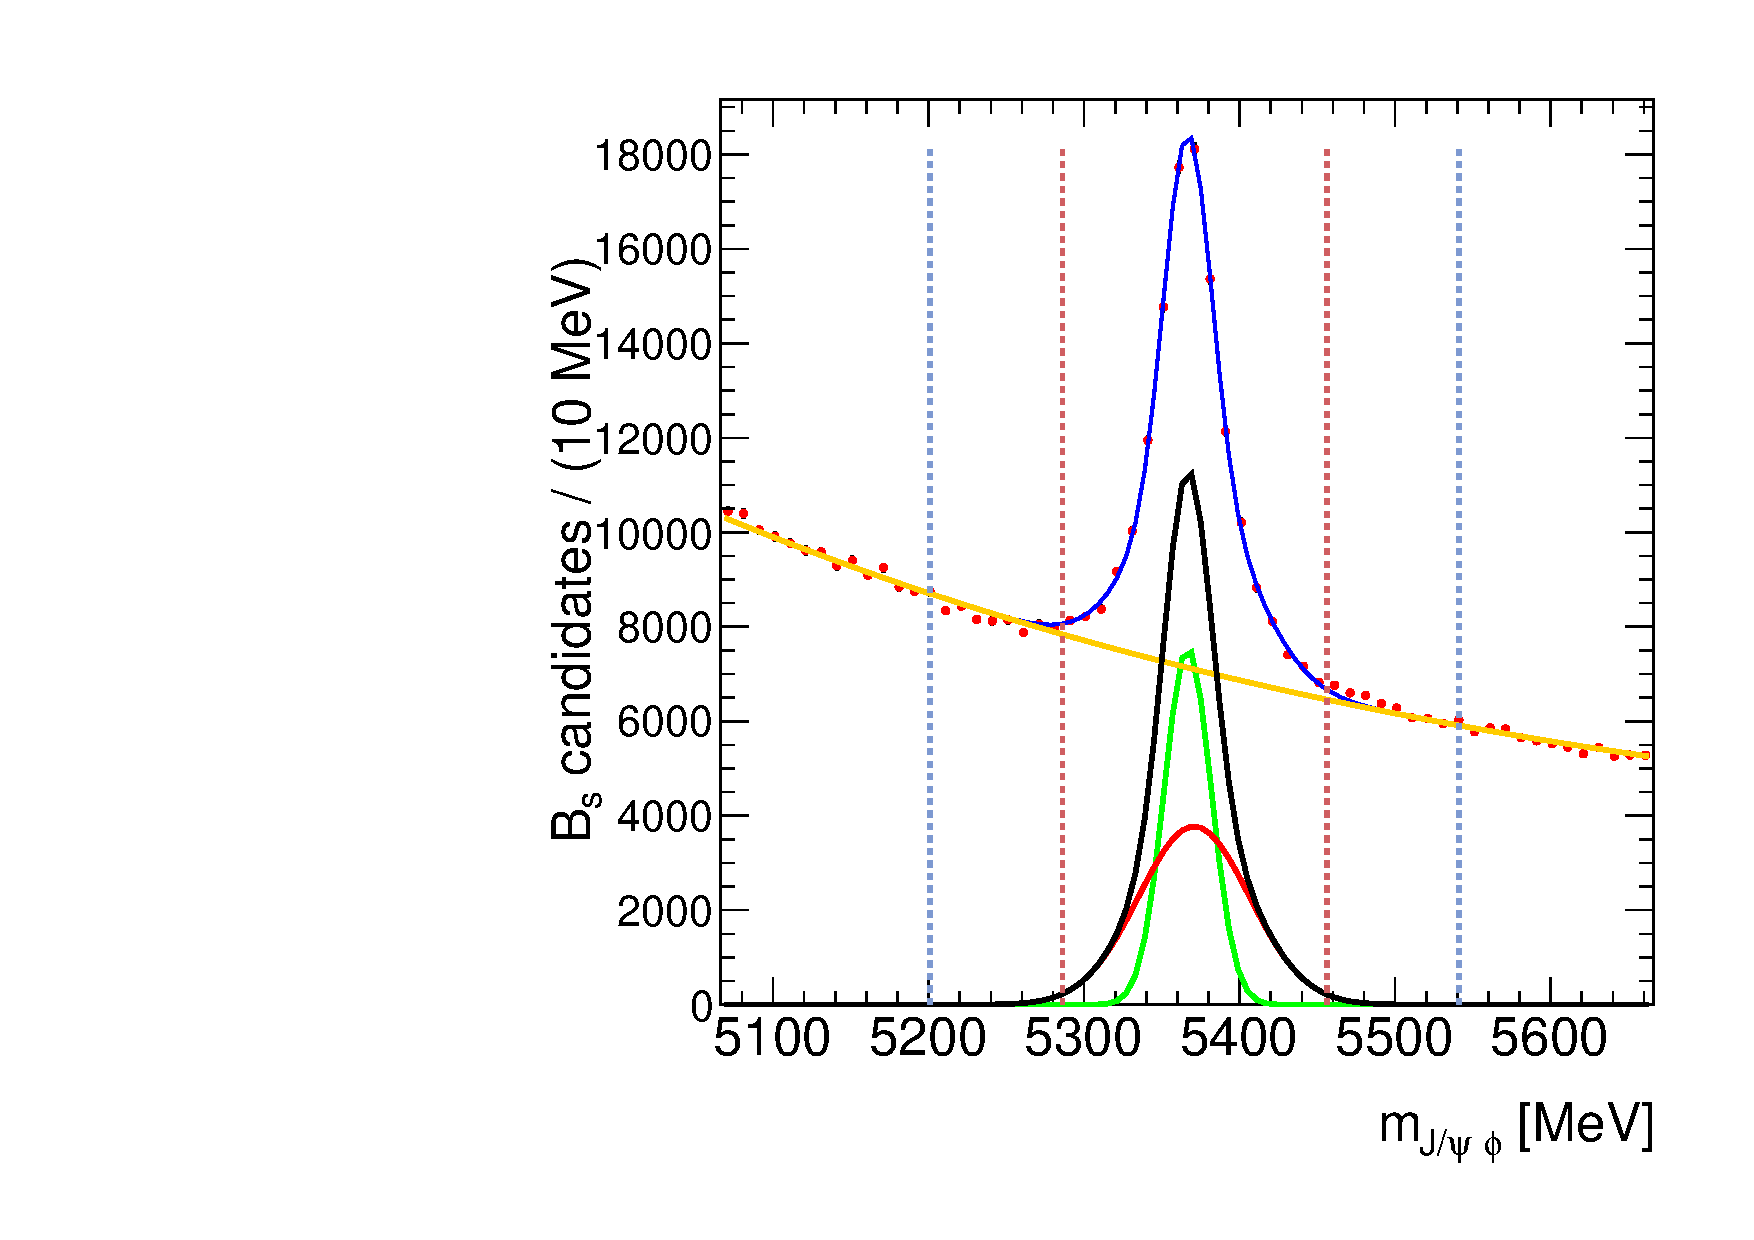
\includegraphics[width=0.47\textwidth]{figures/InternalNote_DataMCComparison/Bs/bsjpsiphibinnedfit.pdf}
\caption{Fit to the invariant mass distribution of \BsJpsiPhi\ events.}
\label{fig:jpsiphi}
\end{center}
\end{figure}

The data/MC comparisons of \pt{} and $\eta{}$ distributions for the \Bs\ are
shown in Figure~\ref{fig:xcheckcompBs}, while the distributions of few
discriminating variables are shown in Figure~\ref{fig:jpsiphivars}..
Finally the distribution of the continuum BDT variable is shown in
Figure~\ref{fig:jpsiphiBDT}.
The signal distributions in data are obtained by subtracting the
sideband shapes in each variable.

\yel[t.b.d.]{Additional studies of the} \BsJpsiPhi are presented in Section~\ref{sec:jpsiphi}.

\begin{figure}[!htb]
\begin{center}
\hspace*{-0.6cm}
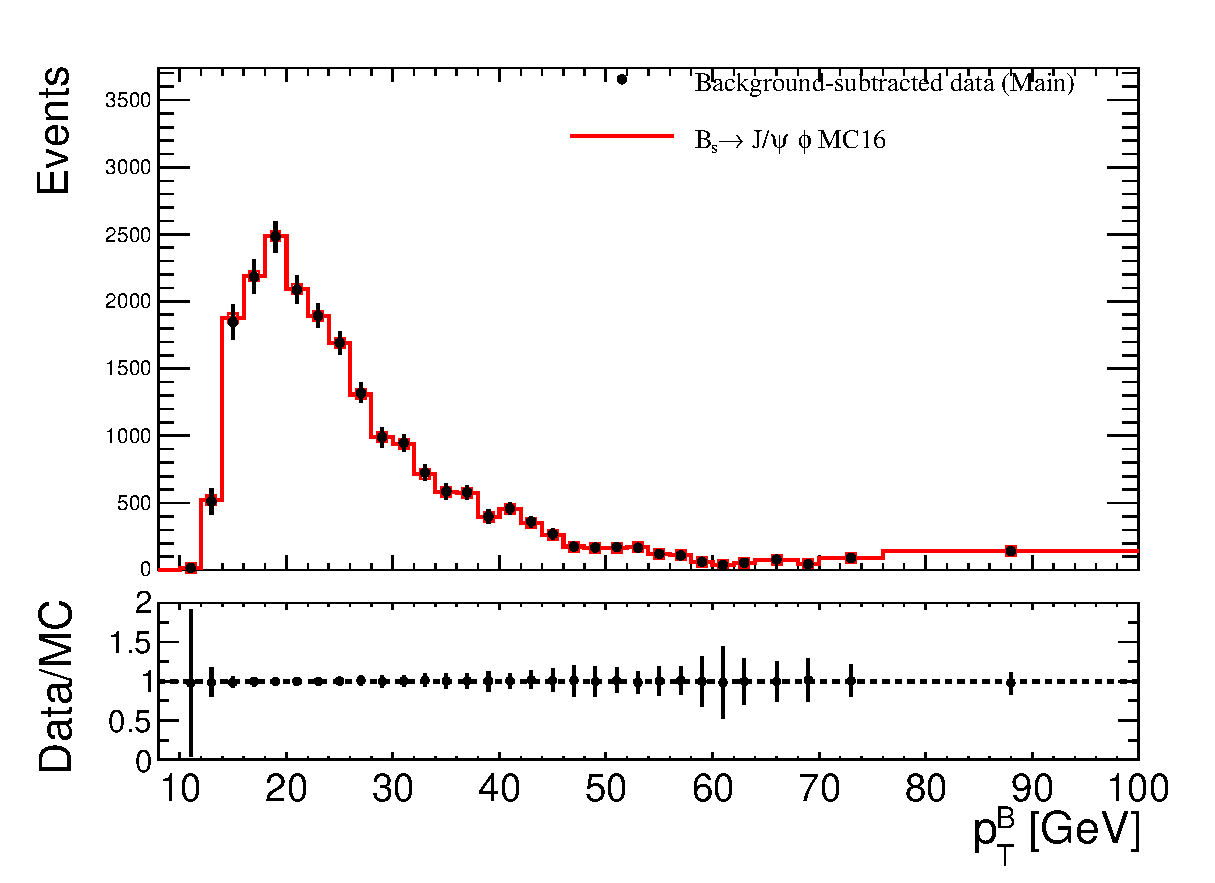
\includegraphics[width=0.52\textwidth]{figures/InternalNote_DataMCComparison/Bs/bsjpsiphi_pT.eps}
\hspace*{-0.6cm}
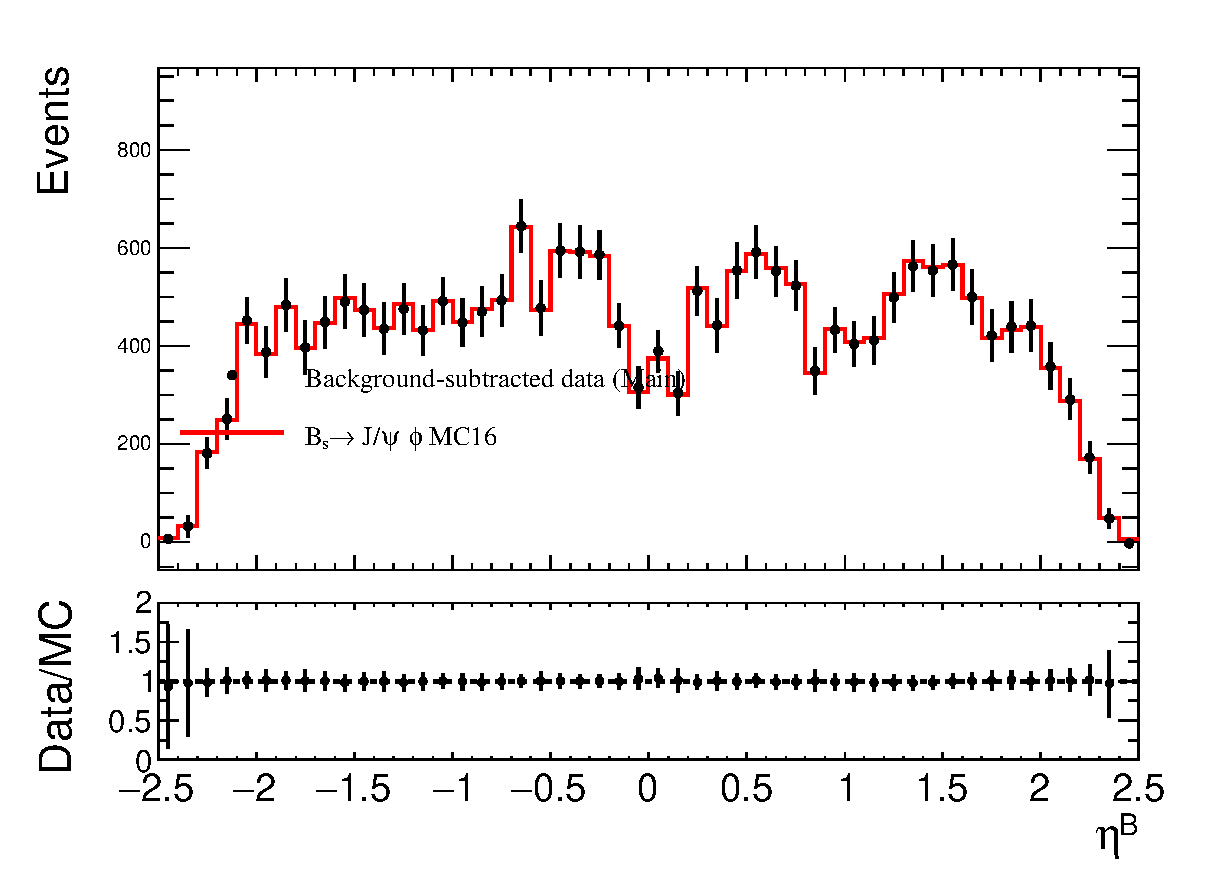
\includegraphics[width=0.52\textwidth]{figures/InternalNote_DataMCComparison/Bs/bsjpsiphi_eta.eps}
\caption{Cross-check on the \pt$^B$ and $\eta^B$ distributions of
the $J/\psi \phi$ candidates in data and signal MC.
The black dots correspond to the sideband subtracted data, while 
the red histograms correspond to reweighted MC 
normalised to the number of data events.}
\label{fig:xcheckcompBs}
\end{center}
\end{figure}
%
\begin{figure}[!htb]
\begin{center}
\hspace*{-0.5cm}
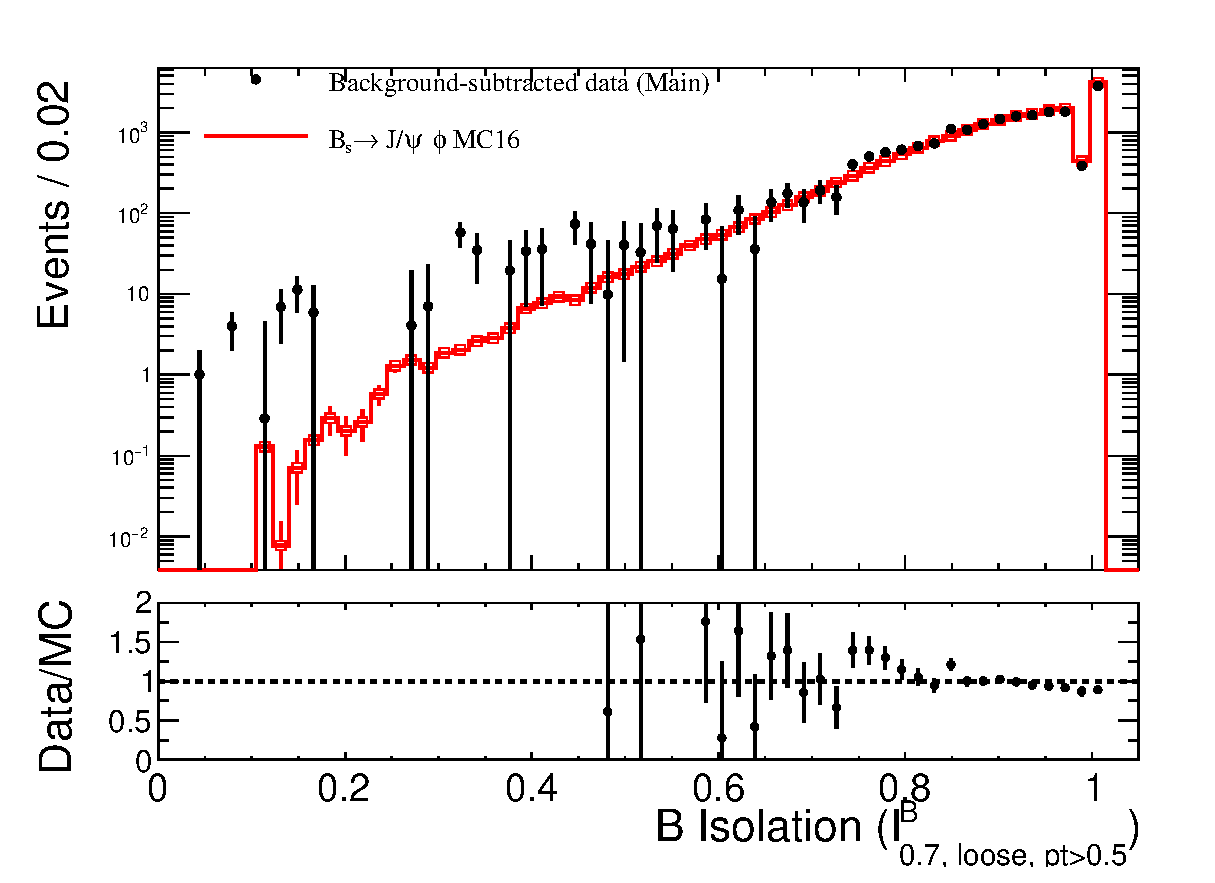
\includegraphics[width=0.48\textwidth]{figures/InternalNote_DataMCComparison/Bs/bsjpsiphi_iso.eps}
\hspace*{-0.5cm}
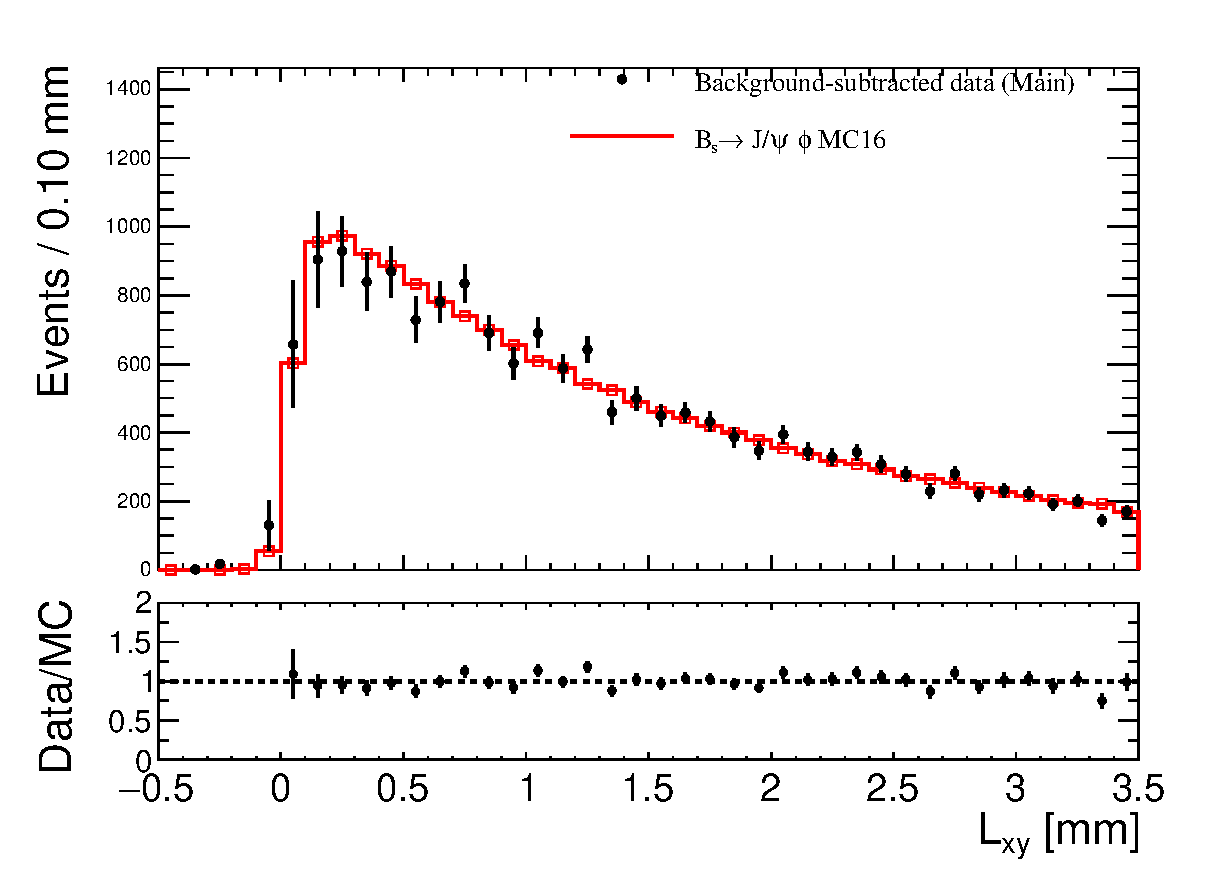
\includegraphics[width=0.48\textwidth]{figures/InternalNote_DataMCComparison/Bs/bsjpsiphi_Lxy.eps}\\
\hspace*{-0.5cm}
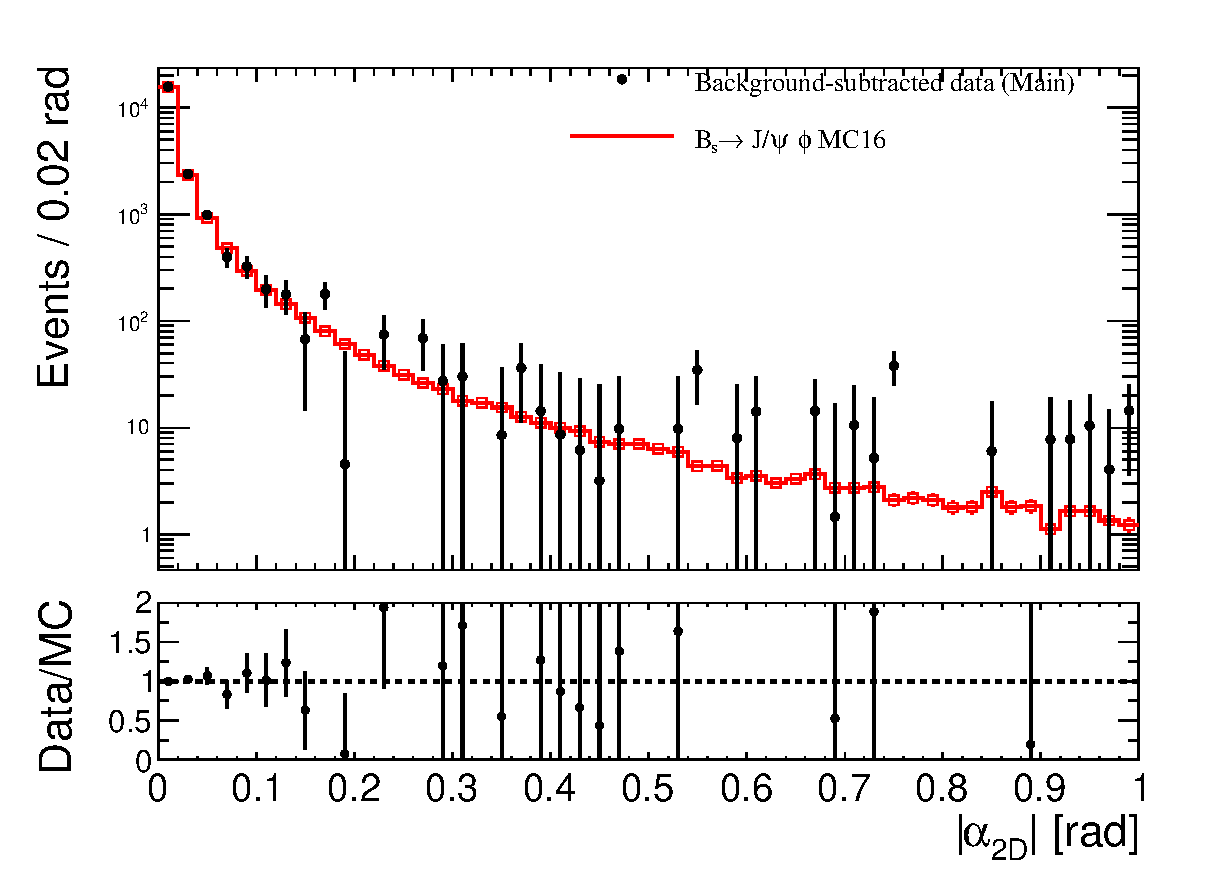
\includegraphics[width=0.48\textwidth]{figures/InternalNote_DataMCComparison/Bs/bsjpsiphi_a2D.eps}
\hspace*{-0.5cm}
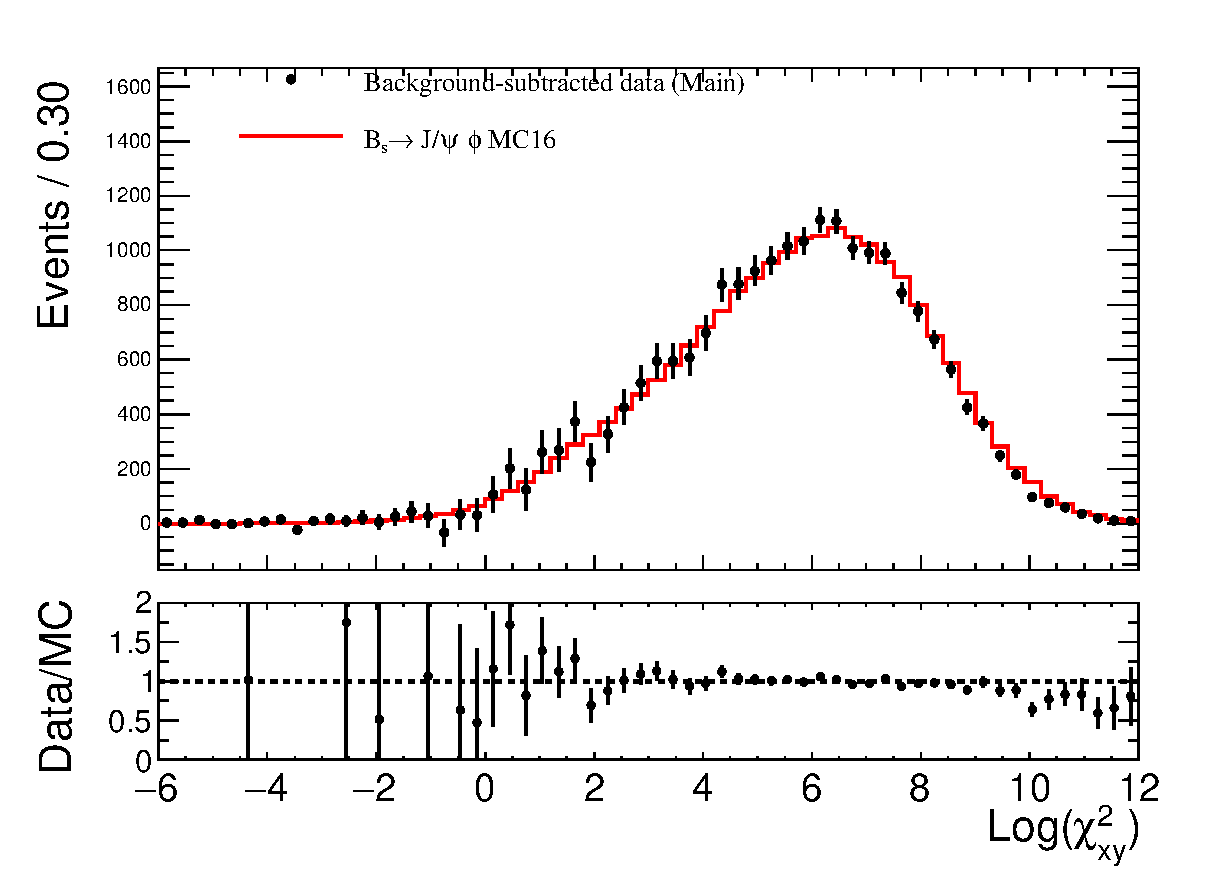
\includegraphics[width=0.48\textwidth]{figures/InternalNote_DataMCComparison/Bs/bsjpsiphi_chi2PVSV.eps}
\caption{{\it{From left to right, from top to bottom}}: 
Data and signal MC distributions of \BsJpsiPhi\ events for the $B$ isolation variable, 
the transverse decay length ($L_{xy}$), $|\alpha_{2D}|$ and 
$\chi^{2}_{xy}$ that represents the separation between production
(PV) and decay (SV) vertices.
The black dots correspond to the sideband subtracted data, while 
the red points correspond to reweighted MC normalised to the number
of data events.}
\label{fig:jpsiphivars}
\end{center}
\end{figure}
%
\begin{figure}[!b]
\begin{center}
\hspace*{-0.4cm}
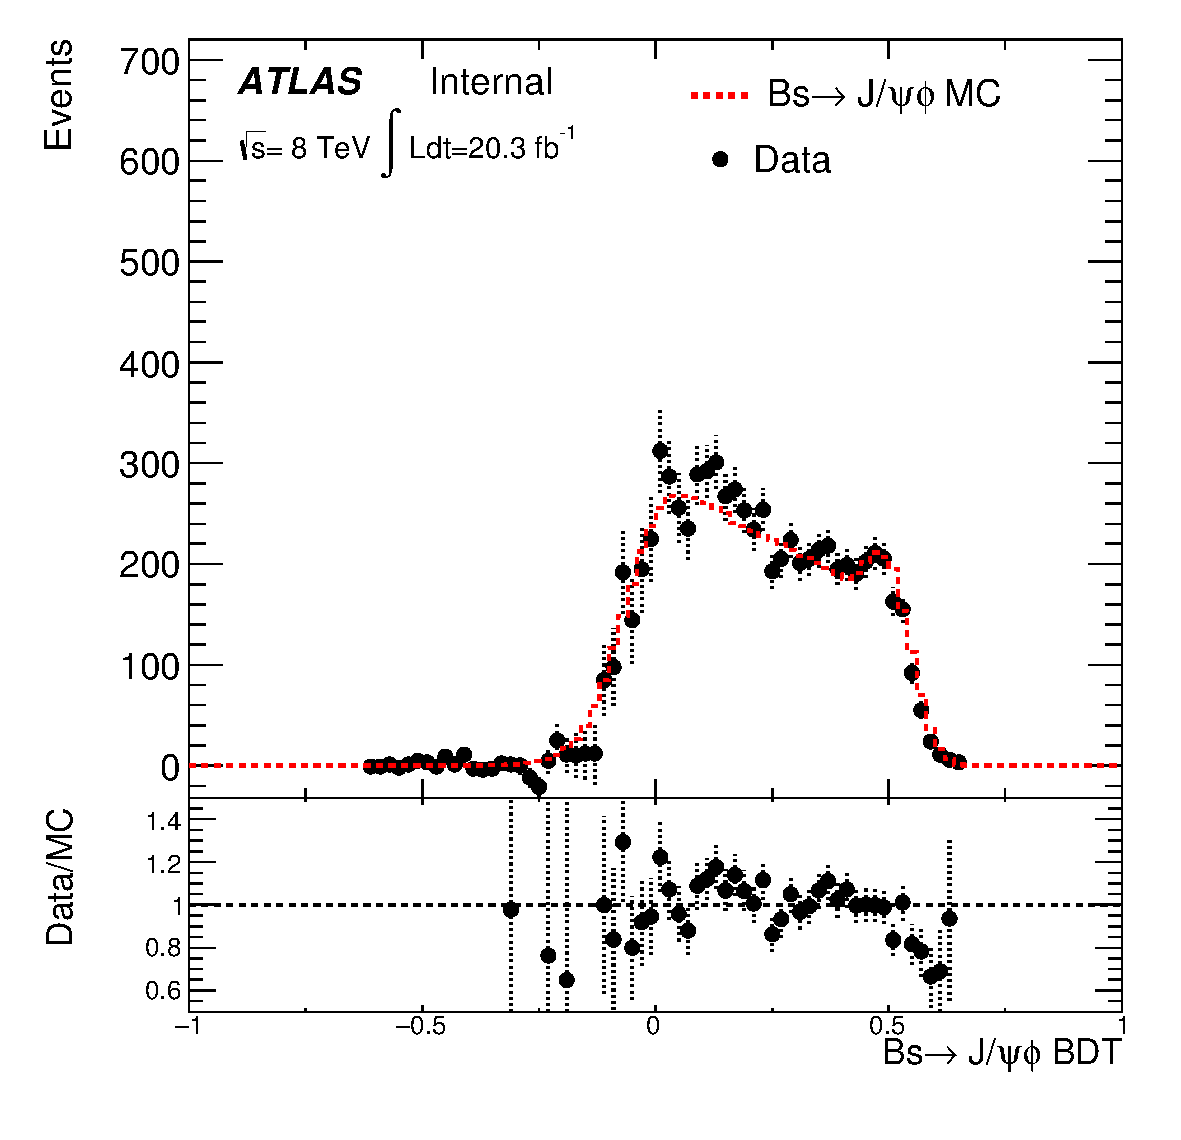
\includegraphics[width=0.47\textwidth]{figures/InternalNote_DataMCComparison/compRun1/Bs/BsJpsiphi_BDT12.pdf}
\hspace*{-0.4cm}
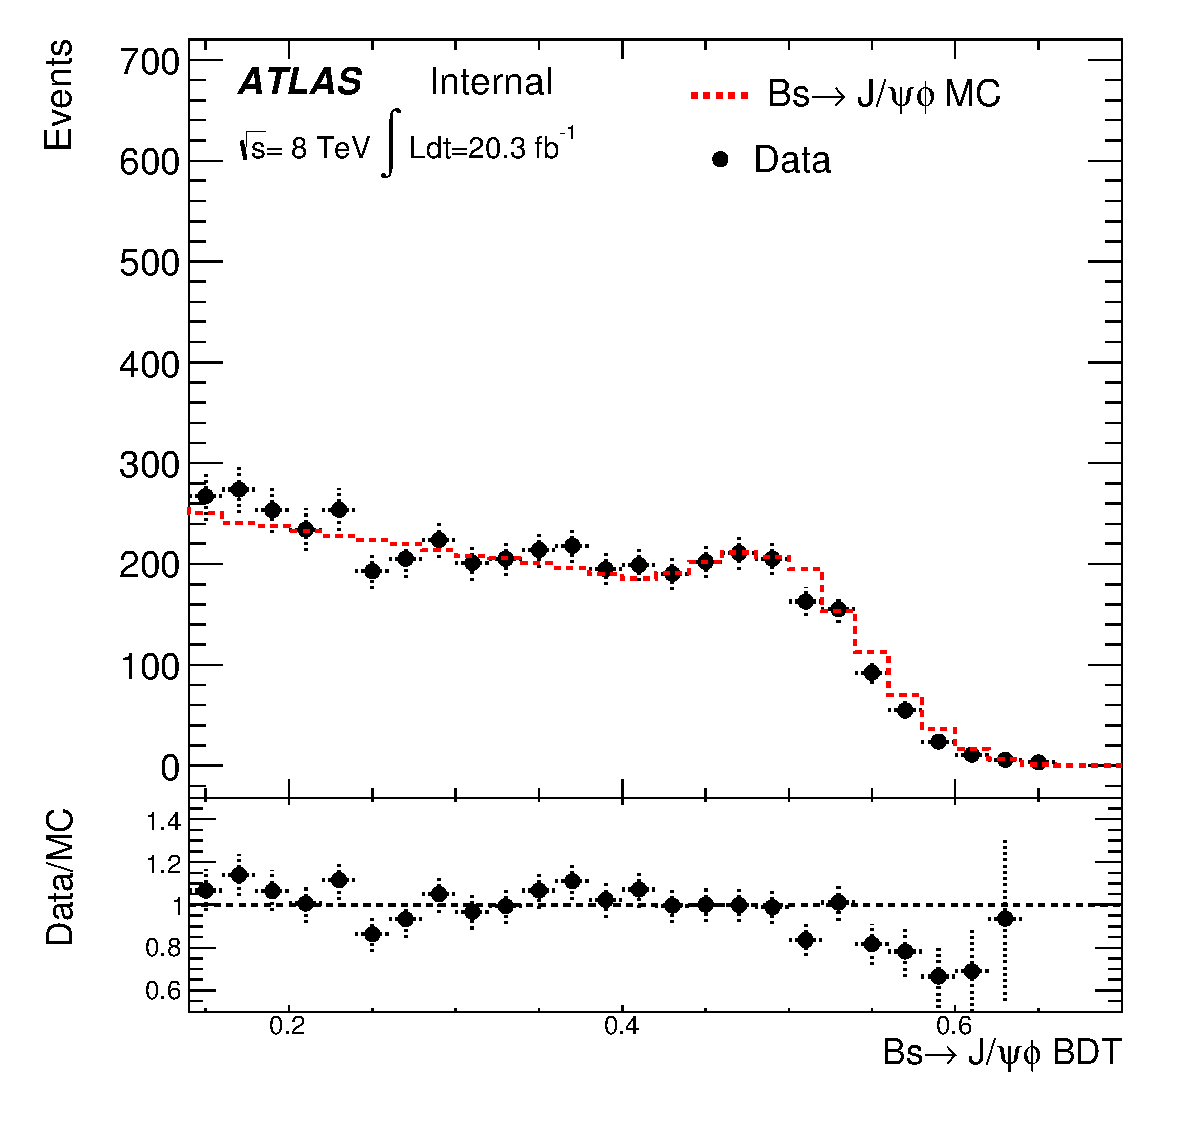
\includegraphics[width=0.47\textwidth]{figures/InternalNote_DataMCComparison/compRun1/Bs/BsJpsiphi_BDT12zoomed.pdf}
\caption{\textbf{Run 1 result, t.b.u.!}Data and signal MC distribution in \BsJpsiPhi\ events for the
continuum BDT variable.
The black dots correspond to the sideband subtracted data, while 
the red points correspond to reweighted MC normalised to the number
of data events. The left plot shows the same distribution zoomed
in the region of interest of the analysis.}
\label{fig:jpsiphiBDT}
\end{center}
\end{figure}
%
%BsJpsiphi_valid2_DR.pdf
 
\subsection{Yield stability during run}
\label{sec:stability}
The stability of the gain in the \Bs sidebands in the 2015 and 2016 data taking periods is shown in Figure~\ref{fig:gainstability}. The gain is calculated as the yield of events per period divided by the luminosity in that period. The gain appears to be stable during the run, within statistical uncertainties.
%The main variations correspond to the increase in trigger efficiency with the introduction of the L2StarB algorithm,
%occurring at 1.36~fb$^{-1}$ in the charged mode and at 6.19~fb$^{-1}$ in the neutral one.
\begin{figure}[!htb]
\begin{center}
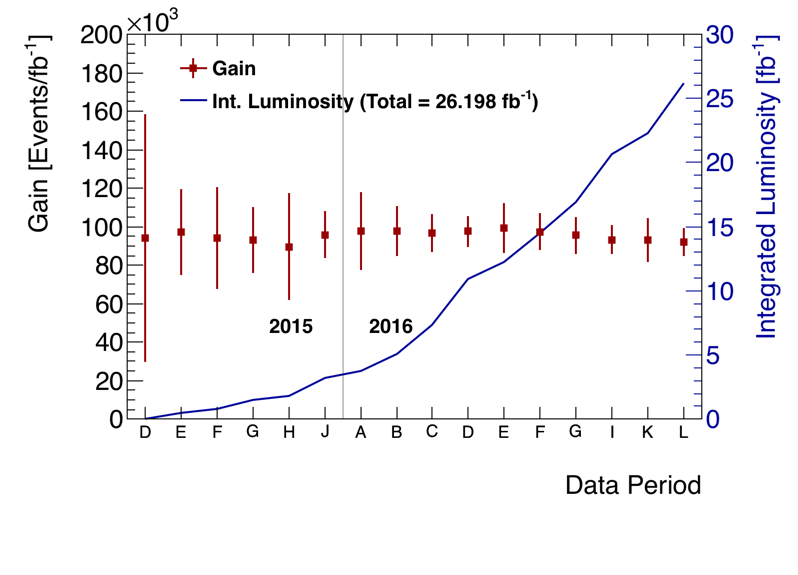
\includegraphics[width=0.7\textwidth]{figures/InternalNote_DataMCComparison/comp/GainPlot.png}
% \hspace*{-0.4cm}
% 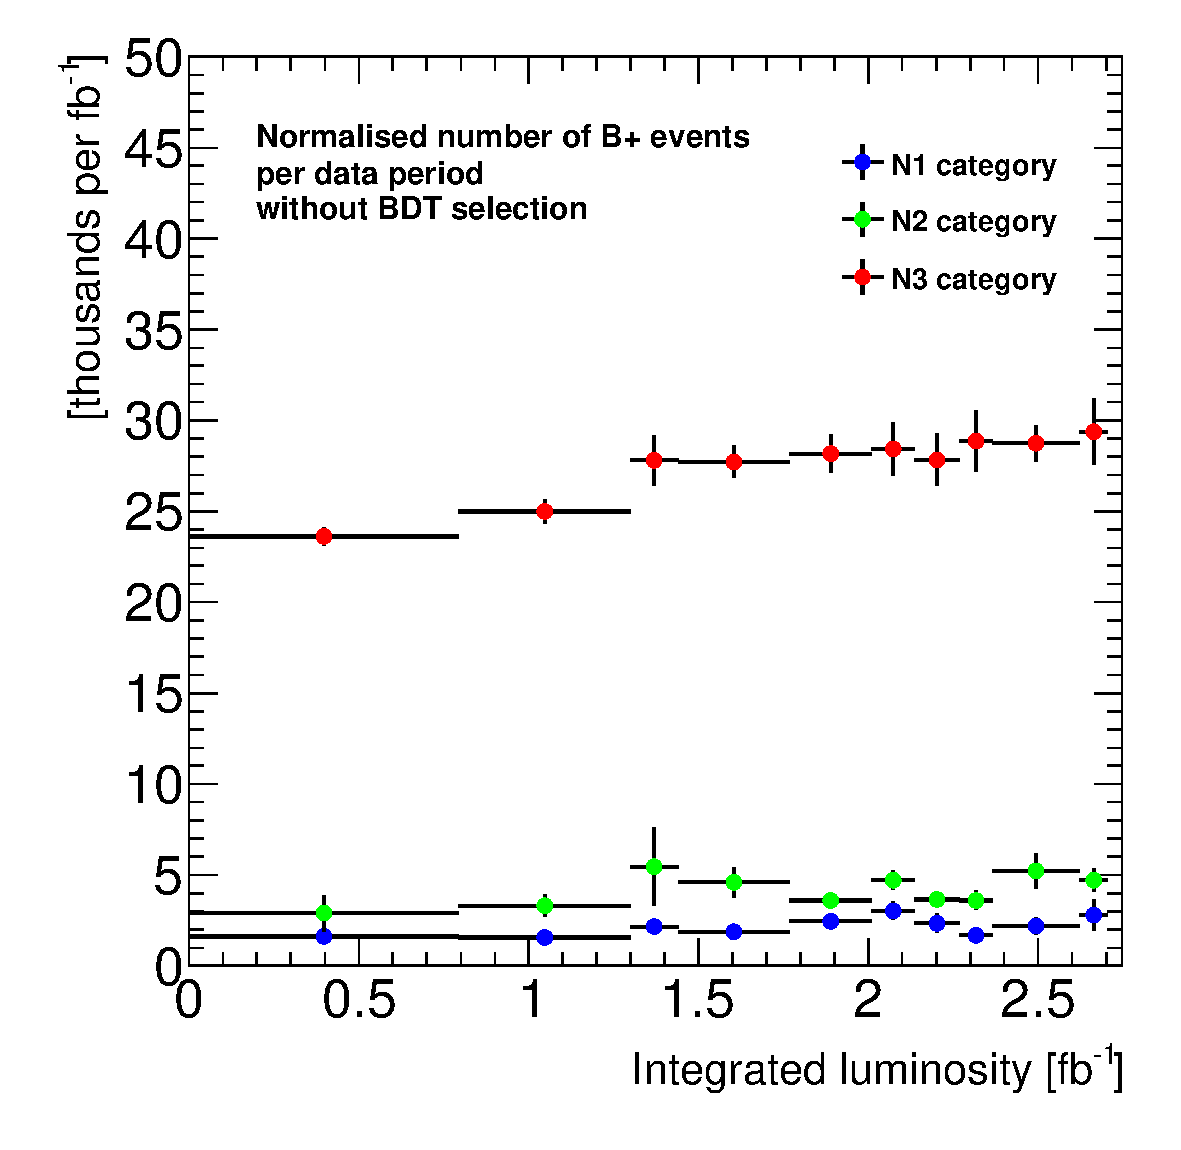
\includegraphics[width=0.47\textwidth]{figures/InternalNote_DataMCComparison/compRun1/Bplus-per-period.pdf}
% \hspace*{-0.4cm}
% 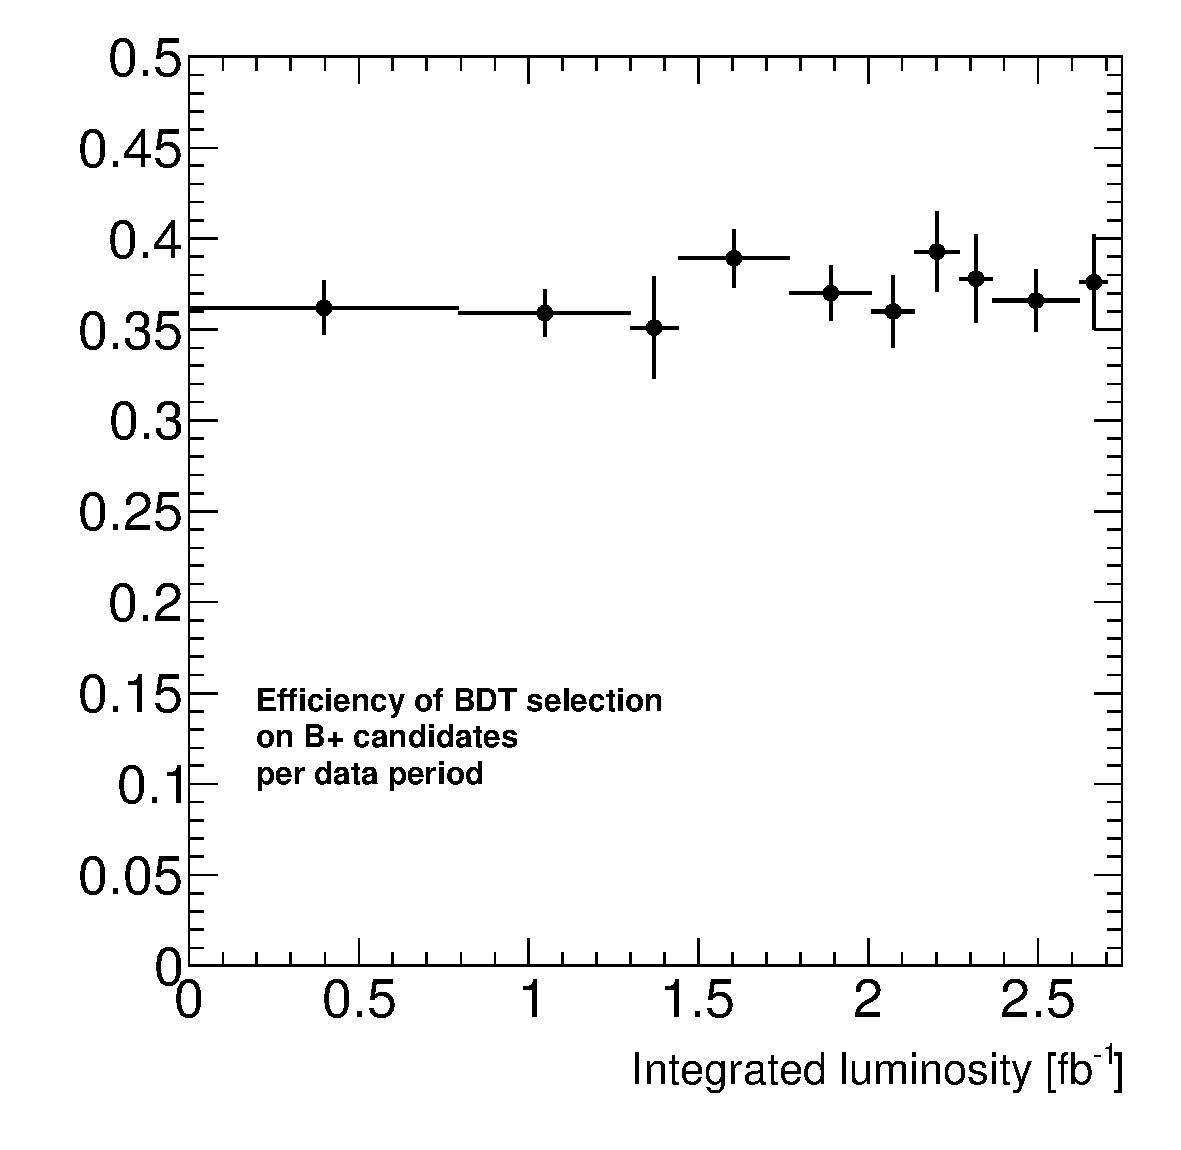
\includegraphics[width=0.47\textwidth]{figures/InternalNote_DataMCComparison/compRun1/Bplus-BDTeff-per-period.pdf}\\
% \hspace*{-0.4cm}
% 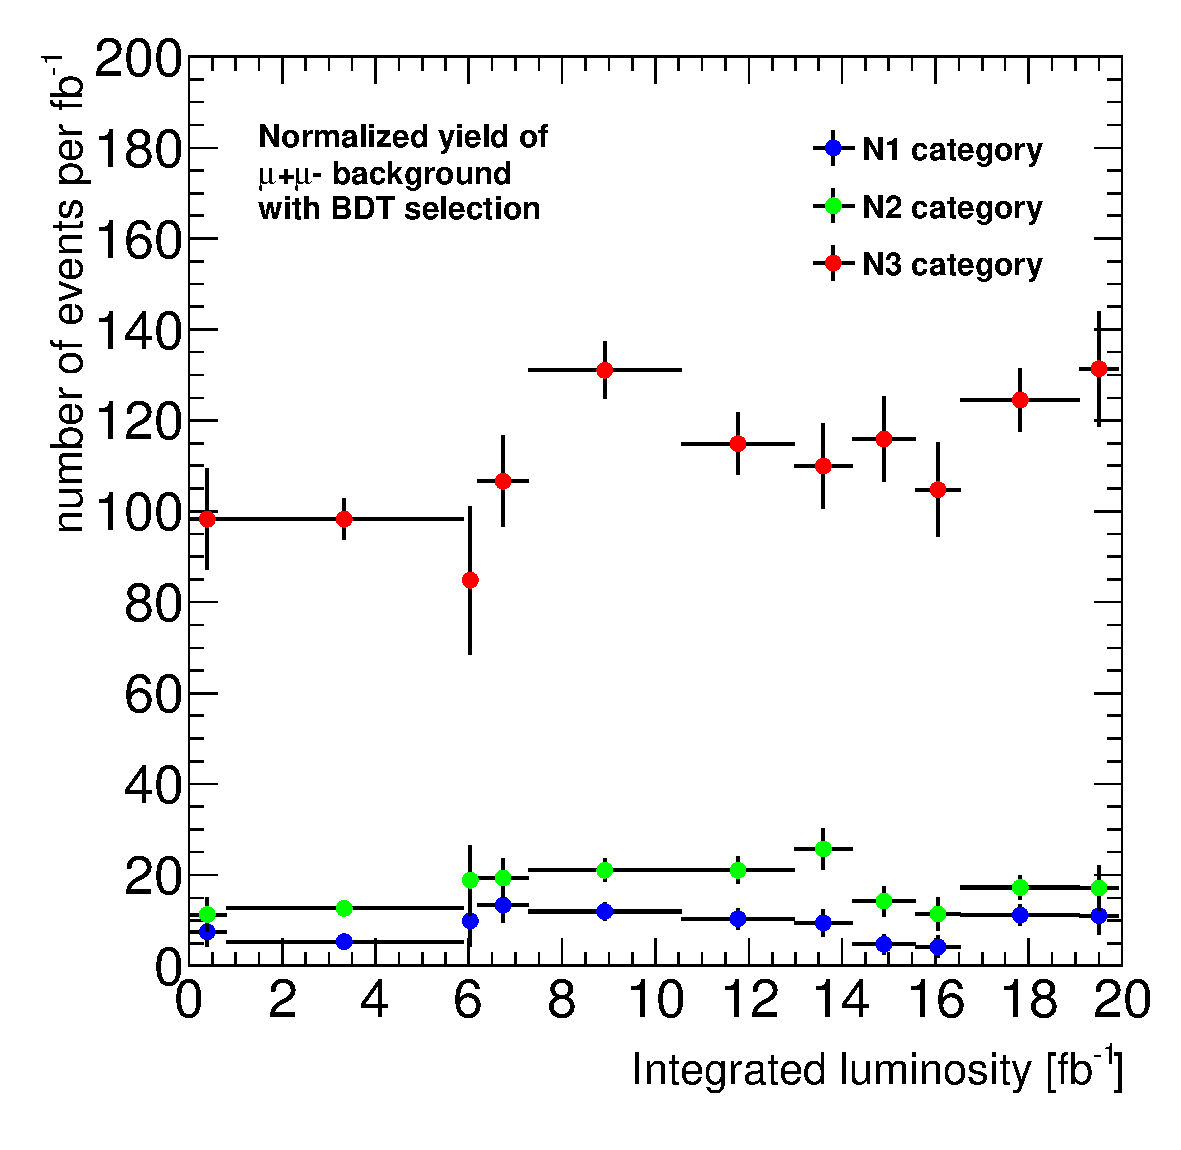
\includegraphics[width=0.47\textwidth]{figures/InternalNote_DataMCComparison/compRun1/Bs-per-period.pdf}
% \hspace*{-0.4cm}
% 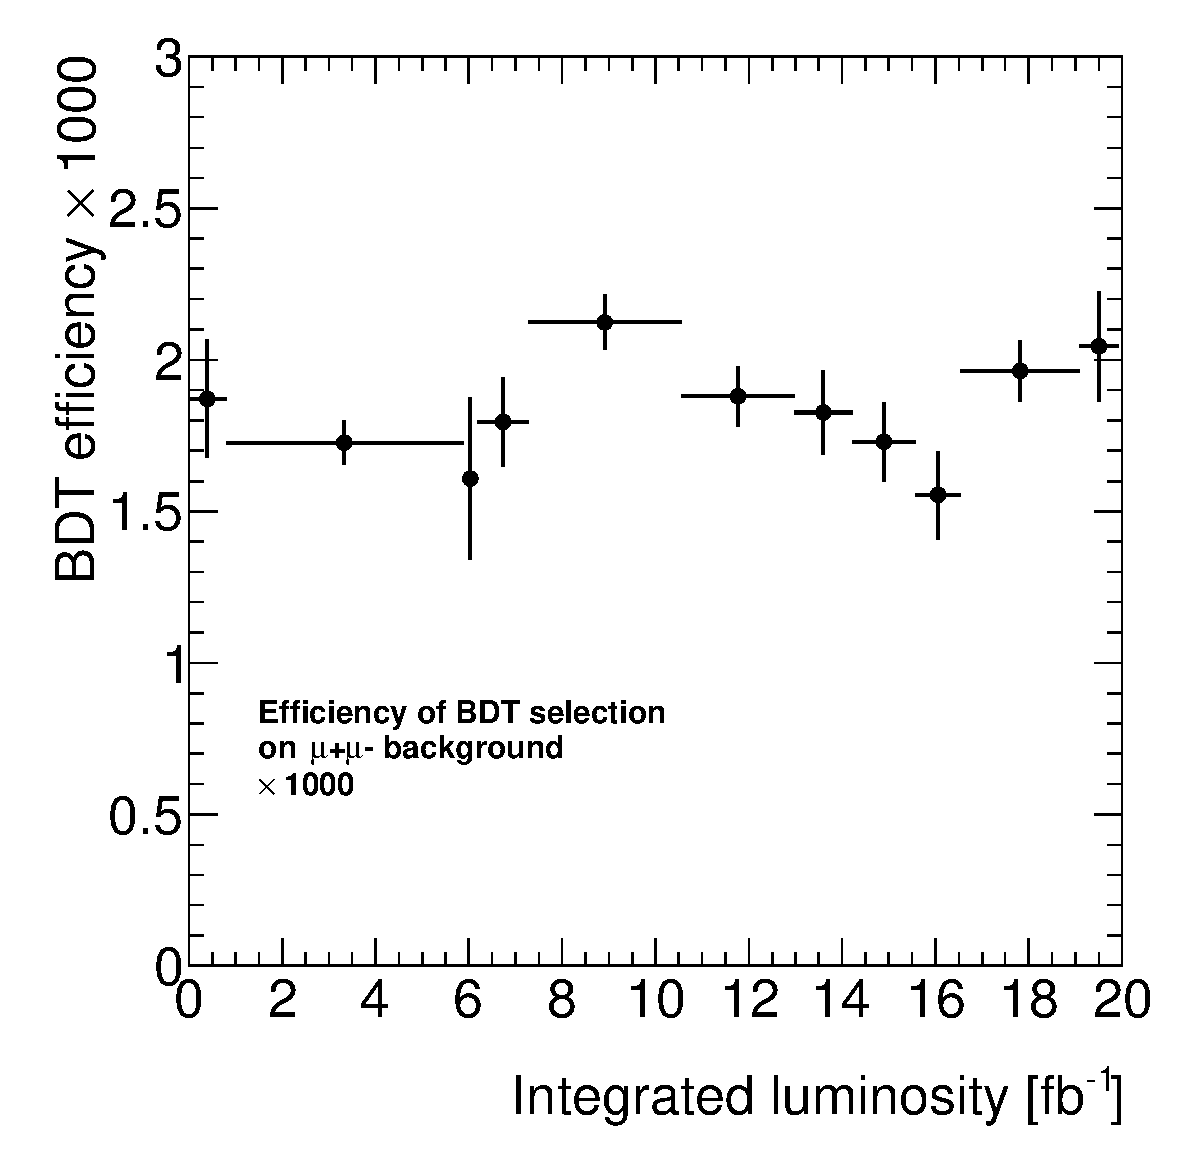
\includegraphics[width=0.47\textwidth]{figures/InternalNote_DataMCComparison/compRun1/Bs-BDTeff-per-period.pdf}
\caption{Stability of \Bs\ gain for 2015 and 2016 data taking periods. Also shown is the integrated luminosity for the analysis when the HLT\_mu4\_mu6\_bBmumu and HLT\_mu4\_mu6\_bBmumu\_Lxy0 triggers are applied to the 2015 and 2016 data respectively.}
\label{fig:gainstability}
\end{center}
\end{figure}


\clearpage
